%%%%%%%%%%%%%%%%%%%%%%%%%%%%%%%%%%%%%%%%%%%%%%%%%%%%%%%%%%%%%%%%%%%%%%%%% 
% $Id: HOFEM_2D_emulation_tr.tex,v 1.4 2022/11/08 14:28:02 luise Exp luise $
% %%%%%%%%%%%%%%%%%%%%%%%%%%%%%%%%%%%%%%%%%%%%%%%%%%%%%%%%%%%%%%%%%%%%%%%%%
%
% Transparencias para reunión de seguimiento HOFEM-AIRBUS sobre "2D
% Emulation" en HOFEM
%
% %%%%%%%%%%%%%%%%%%%%%%%%%%%%%%%%%%%%%%%%%%%%%%%%%%%%%%%%%%%%%%%%%%%%%%%%%
% Magia para que el acrobat reader lea bien el documento.
%\pdfobjcompresslevel=1

%\documentclass[notes,smaller,xcolor=table,dvipsnames]{beamer}
\documentclass[smaller,xcolor=table,dvipsnames]{beamer}

%\documentclass[notes,smaller,xcolor=table,dvipsnames,trans]{beamer}
%\documentclass[smaller,xcolor=table,dvipsnames,trans]{beamer}

%documentclass[notes,smaller,xcolor=table,dvipsnames,handout,hyperref={bookmarks=false}]{beamer}
%\documentclass[smaller,xcolor=table,dvipsnames,handout,hyperref={bookmarks=false}]{beamer}

%Ver uso de oprion onlyslideswithnotes  que no me parece funcionar

%\hypersetup{colorlinks=true,linkcolor=purple}
%\hypersetup{colorlinks=true,allcolors=purple}

%\includeonlyframes{current}

\mode<handout>
{
  \usepackage{pgfpages}
%  \pgfpagesuselayout{2 on 1}[a4paper,border shrink=5mm]
%  \pgfpagesuselayout{4 on 1}[a4paper,landscape,border shrink=5mm]
  \nofiles
}

\usepackage{ifthen}
% \newboolean{ARCS} % Requiere package ``ifthen''
% \setboolean{ARCS}{FALSE} % Si true se personaliza algo para el curso
%                         % ARCS (antennas and RCS del MasteEADS)


% %%%%%%%%%%%%%%%%%%%%%%%%%%%%%%%%%%%%%%%%%%%%%%%%%%%%%%%%%%%%%%%%%%%%%%%%%

% $Id$

% %%%%%%%%%%%%%%%%%%%%%%%%%%%%%%%%%%%%%%%%%%%%%%%%%%%%%%%%%%%%%%%%%%%%%

% Estilo de los últimos años con linea azul al borde

% \mode<presentation>
% {
% %  \usetheme{Warsaw}
%   \usetheme{Boadilla}

%   \setbeamercovered{transparent}
%   % or whatever (possibly just delete it)

% \setbeamertemplate{navigation symbols}{}

% }

% \useoutertheme{uc3mcourse_updated2020} % curso de uc3m

% %%%%%%%%%%%%%%%%%%%%%%%%%%%%%%%%%%%%%%%%%%%%%%%%%%%%%%%%%%%%%%%%%%%%%

% Estilo de Sergio en traspas Radar, campos, etc

\usetheme{uc3m}


% %%%%%%%%%%%%%%%%%%%%%%%%%%%%%%%%%%%%%%%%%%%%%%%%%%%%%%%%%%%%%%%%%%%%%


%\setbeameroption{show notes on second screen=bottom}

%\setbeamersize{text margin right=0.1\linewidth,text margin left=0.1\linewidth}

\setbeamertemplate{frametitle continuation}[from second]

% \usepackage[spanish,es-noquoting,es-nolists,es-noshorthands]{babel}
%  \decimalpoint % utilizamos punto como separador decimal
%  \deactivatetilden % Desactiva abreviaciones ~n y ~N que dan muchos problemas.
% % %                Por ejemplo, con abreviaciones de bibtex como M.~N. Vouvakis
\usepackage[english]{babel}
% or whatever

% Tikz y derivados
%\input{preamble_tr_tikz}

%\usepackage[latin1]{inputenc}
\usepackage[utf8]{inputenc}
% or whatever

%\usepackage[T1]{fontenc}
% Or whatever. Note that the encoding and the font should match. If T1
% does not look nice, try deleting the line with the fontenc.
%\usepackage{times}
%\usepackage{lmodern}


\usepackage{amsmath}
\usepackage{amssymb}
%\usepackage{amscd} % conmutative diagrams
\usepackage{latexsym}

\usepackage{pifont}


\usepackage{verbatim}
\usepackage{listings}

  \lstdefinestyle{myFORTRANcode}
    {language=[90]Fortran,
    basicstyle=\ttfamily\footnotesize,
    keywordstyle=\color{blue}\ttfamily,
    stringstyle=\color{brown}\ttfamily,
    commentstyle=\color{red}\ttfamily,
    tabsize=2,
%    frame=single,
%    backgroundcolor=\color{yellow},
    breaklines=true,breakatwhitespace=true,prebreak=\space\&
  }
  \lstdefinestyle{myFORTRANcodeS} % S as "small"
    {language=[90]Fortran,
    basicstyle=\ttfamily\scriptsize,
    keywordstyle=\color{blue}\ttfamily,
    stringstyle=\color{brown}\ttfamily,
    commentstyle=\color{red}\ttfamily,
    tabsize=2,
%    frame=single,
%    backgroundcolor=\color{yellow},
    breaklines=true,breakatwhitespace=true,prebreak=\space\&
  }

  \lstdefinestyle{myFORTRANcodeOpenMP}
    {language=[90]Fortran,
    basicstyle=\ttfamily\footnotesize,
    keywordstyle=\color{blue}\ttfamily,
    stringstyle=\color{brown}\ttfamily,
    commentstyle=\color{red}\ttfamily,
    morecomment=[l]{\$},
    tabsize=2,
%    frame=single,
%    backgroundcolor=\color{yellow},
    breaklines=true,breakatwhitespace=false,prebreak=\space\&
  }


\usepackage{graphicx}
\usepackage{subfig}
%\usepackage{subfigure}


\usepackage{xmpmulti}

\usepackage{notacion}

% \usepackage{def_listas}

\usepackage{pdfpages}

\usepackage{multimedia}

\usepackage{array}  % Para tablas
\newcolumntype{C}{>{$}c<{$}} % Identificadores de columna en math mode
\newcolumntype{L}{>{$}l<{$}}
\newcolumntype{R}{>{$}r<{$}}

%\setlength{\arrayrulewidth}{0.5mm}
%\setlength{\tabcolsep}{18pt}
\setlength{\tabcolsep}{10pt}
\renewcommand{\arraystretch}{1.5}


\newcommand{\vbs}{\vspace{\baselineskip}}
\newcommand{\vbss}{\vspace{0.5\baselineskip}}
\newcommand{\vbsf}{\vspace*{\baselineskip}}
\newcommand{\vbssf}{\vspace*{0.5\baselineskip}}
\newcommand{\FIGURA}[1]{\vspace*{2\baselineskip} \centering{FIGURA \\ #1} \vspace*{2\baselineskip} }


\newcommand{\crule}{{\color{cyan} \hrule} }

\setcounter{tocdepth}{4}

% El paquete enumitem redefine las listas de Beamer:
%\usepackage{enumitem}
% \setitemize{label=\usebeamerfont*{itemize item}%
%    \usebeamercolor[fg]{itemize item}
%    \usebeamertemplate{itemize item}}

% Alternativa:
\newcounter{saveenumi}
\newcommand{\seti}{\setcounter{saveenumi}{\value{enumi}}}
\newcommand{\conti}{\setcounter{enumi}{\value{saveenumi}}}
\resetcounteronoverlays{saveenumi}




\newcounter{savedenum}
\newcommand*{\saveenum}{\setcounter{savedenum}{\theenumi}}
\newcommand*{\resumeenum}{\setcounter{enumi}{\thesavedenum}}


% %%%%%%%%%%%%%%%%%%%%%%%%%%%%%%%%%%%%%%%%%%%%%%%%%%%%%%%%%%%%%%%%%%%%%%%%%
%  Líneas para hacer versión con "notes" comentando cada traspa
%  Comentar las líneas para versión sin notes

% \usepackage{pgfpages}

% \setbeamertemplate{note page}[plain]
% \setbeameroption{show notes on second screen=bottom}
% \makeatletter
% \def\beamer@setupnote{%
%   \gdef\beamer@notesactions{%
%     \beamer@outsideframenote{%
%       \beamer@atbeginnote%
%       \beamer@notes%
%       \ifx\beamer@noteitems\@empty\else
%       \begin{itemize}\itemsep=0pt\parskip=0pt%
%         \beamer@noteitems%
%       \end{itemize}%
%       \fi%
%       \beamer@atendnote%
%     }%
%     \gdef\beamer@notesactions{}%
%   }
% }
% \makeatother

% %%%%%%%%%%%%%%%%%%%%%%%%%%%%%%%%%%%%%%%%%%%%%%%%%%%%%%%%%%%%%%%%%%%%%%%%%

\newcommand{\GreenT}{\url{Green3D}}
\newcommand{\GreenD}{\url{Green2D}}
\newcommand{\GreenTEw}{\url{Green3D_Ewald1D}}

% %%%%%%%%%%%%%%%%%%%%%%%%%%%%%%%%%%%%%%%%%%%%%%%%%%%%%%%%%%%%%%%%%%%%%%%%%

% Controla si se genera una version para alumno
% o no. En la version para alumno se omiten algunos detalles
\newboolean{alumno} % Requiere package ``ifthen'' 
%\setboolean{alumno}{TRUE}
\setboolean{alumno}{FALSE}

% %%%%%%%%%%%%%%%%%%%%%%%%%%%%%%%%%%%%%%%%%%%%%%%%%%%%%%%%%%%%%%%%%%%%%%%%%

\newcommand{\dirinputtex}{./inputtex}

\graphicspath{{./figures/}{./figures_Issue_field_tangential_at_PEC_non_zero/}{./Ewald}}
\lstset{inputpath=./code_output}

\usepackage[nofancy]{rcsinfo}
\rcsInfo $Id: HOFEM_2D_emulation_tr.tex,v 1.4 2022/11/08 14:28:02 luise Exp luise $
% %%%%%%%%%%%%%%%%%%%%%%%%%%%%%%%%%%%%%%%%%%%%%%%%%%%%%%%%%%%%%%%%%%%%%%%%%


\title[HOFEM-AIRBUS(v{\rcsInfoRevision})]{HOFEM-AIRBUS 2D Emulation}

%\date[]{}%{Version {\rcsInfoRevision}, checked out \today}

% \author[GREMA-TSC-UC3M]{Luis E.\ Garcia-Castillo \\
%   \url{legcasti@ing.uc3m.es}}

\author[]{-June 7th 2022---}

\author{}

\date[]{\small{%
    Group of Radiofrequency, Electromagnetism, Microwaves \\ and Antennas (GREMA) \\    \url{http://grema.webs.tsc.uc3m.es/}
 \\[0.8\baselineskip]
    % 
    Departamento de Teoría de la Señal y Comunicaciones (TSC) \\
    Universidad Carlos III de Madrid, Spain \\
  }}

% \date[]{\small{%
%     Departamento de Teoría de la Señal y Comunicaciones (TSC) \\
%     Universidad Carlos III de Madrid, Spain \\
% }}

\institute{Contact: Luis Emilio García-Castillo
  \url{legcasti@ing.uc3m.es}, Adrián Amor \url{aamor@ing.uc3m.es}, Sergio Llorente \url{sollorent@ing.uc3m.es}}

%\date{}

% %%%%%%%%%%%%%%%%%%%%%%%%%%%%%%%%%%%%%%%%%%%%%%%%%%%%%%%%%%%%%%%%%%%%%%%%%

% If you have a file called "university-logo-filename.xxx", where xxx
% is a graphic format that can be processed by latex or pdflatex,
% resp., then you can add a logo as follows:

% \pgfdeclareimage[height=0.5cm]{university-logo}{university-logo-filename}
% \logo{\pgfuseimage{university-logo}}



% Delete this, if you do not want the table of contents to pop up at
% the beginning of each section:
% \AtBeginSection[]
% {
%   \begin{frame}<beamer>[allowframebreaks]{Outline}
%     \tableofcontents[currentsection]
%   \end{frame}
% }
% \AtBeginSubsection[]
% {
%   \begin{frame}<beamer>{Outline}
%     \tableofcontents[currentsection,currentsubsection]
%   \end{frame}
% }

%\AtBeginPart{\frame{\partpage}}

% If you wish to uncover everything in a step-wise fashion, uncomment
% the following command: 

%\beamerdefaultoverlayspecification{<+->}

% %%%%%%%%%%%%%%%%%%%%%%%%%%%%%%%%%%%%%%%%%%%%%%%%%%%%%%%%%%%%%%%%%%%%%%%%%%%%

% Ya esta definido comando en el fichero de preambulo.
% \newcommand{\FIGURA}[1][]{\vspace*{2\baselineskip}\alert{FIGURA!!!} #1\vspace*{2\baselineskip}}

% %%%%%%%%%%%%%%%%%%%%%%%%%%%%%%%%%%%%%%%%%%%%%%%%%%%%%%%%%%%%%%%%%%%%%%%%%%%%


  \newcommand*{\meshCCC}[3]{cylinder_sp_circled_s_circled_d_#1_h_#2_m_#3.em.mesh}
  \newcommand*{\meshCSS}[3]{cylinder_sp_squared_s_squared_d_#1_h_#2_m_#3.em.mesh}
  \newcommand*{\meshPS}[3]{cylinder_sp_pec_s_squared_d_#1_h_#2_m_#3.em.mesh}
  \newcommand*{\meshPC}[3]{cylinder_sp_pec_s_circled_d_#1_h_#2_m_#3.em.mesh}

\begin{document}

\begin{frame}
  \titlepage
\end{frame}

% \begin{frame}[allowframebreaks]{Outline}
%   \tableofcontents
% \end{frame}


% %%%%%%%%%%%%%%%%%%%%%%%%%%%%%%%%%%%%%%%%%%%%%%%%%%%%%%%%%%%%%%%

  \begin{frame}[plain]
    \centering \Large{We start considering the use of {\GreenT} or
      {\GreenD} the scattering of inifinite cylinders using 3D
      simulator on a section (``slice'') of the cylinder}
    
  \end{frame}

  %%%%%%%%%%%%%%%%%%%%%%%%%%%%%%%%%%%%%%%%%%%%%%%%%%%%%%%%%%%%%%%%%%%%%%%%% 
% $Id$
% %%%%%%%%%%%%%%%%%%%%%%%%%%%%%%%%%%%%%%%%%%%%%%%%%%%%%%%%%%%%%%%%%%%%%%%%%
%
% Set de slides estudiando diferencias entre uso de Green3D o Green2D
% para problema cilindro infinito usando una seccion (rodaja 3D) del
% cilindro
%
% %%%%%%%%%%%%%%%%%%%%%%%%%%%%%%%%%%%%%%%%%%%%%%%%%%%%%%%%%%%%%%%%%%%%%%%%%

% %%%%%%%%%%%%%%%%%%%%%%%%%%%%%%%%%%%%%%%%%%%%%%%%%%%%%%%%%%%%%%%%%%%%%%%%%
\subsection{Green's Function for 2D Emulation}
% %%%%%%%%%%%%%%%%%%%%%%%%%%%%%%%%%%%%%%%%%%%%%%%%%%%%%%%%%%%%%%%%%%%%%%%%%


\begin{frame}[allowframebreaks]{HOFEM 2D Emulation}

  \begin{columns}
    \column{0.25\textwidth} \centering
    {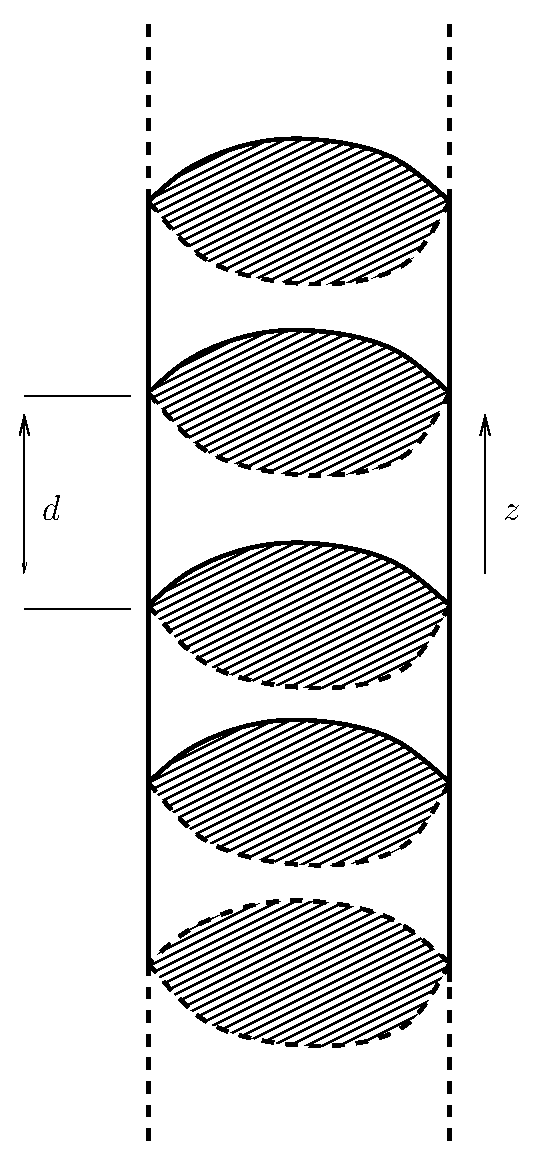
\includegraphics[angle=0,width=\textwidth]{2D_Cylinder_sliced}}

    \column{0.7\textwidth} \centering
    \begin{block}{3D Green's Function}
      \begin{itemize}
      \item Sum of infinite contributions (from each repeated cell)
        
      \item Ewald acceleration needed 
        %
        \begin{equation*}
          \text{Green}(R) = \dfrac{1}{4\pi}
          \sum_{n=-\infty}^\infty \dfrac{e^{-j k R_n}}{R_n}
        \end{equation*}
        with
        \begin{equation*}
          R_n=\abs{\vr-\vrp_n}, \vrp_n=\vrp_0 + n d
        \end{equation*}

        \begin{itemize}
        \item New implementation (for 1D periodicity) required
        \item 1D periodicity case is different (and much more
          involved) than 2D periocicity already present in the code
          for the infinite array.
        \item See details later in Section~\ref{sec:Ewald1D}
        \end{itemize}
      \end{itemize}
      
    \end{block}
  \end{columns}

  \framebreak % %%%%%%%%%%%%%%%%%%%%%%%%%%%%%%%%%%%%%%

  \begin{columns}
    \column{0.25\textwidth} \centering
    {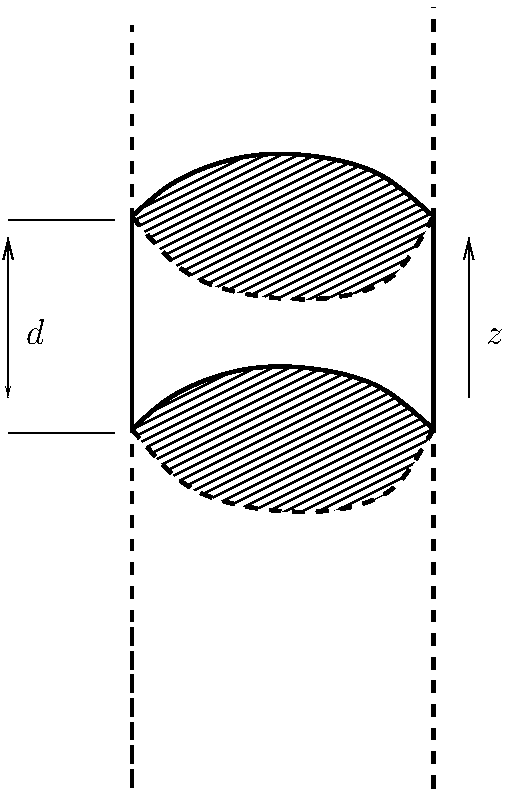
\includegraphics[angle=0,width=\textwidth]{2D_Cylinder_unitslice}}
    
    \column{0.7\textwidth} \centering
    \begin{block}{2D Green's Function}
      \begin{itemize}
      \item No summation needed
        \begin{equation*}
          \text{Green}(\rho) = \dfrac{1}{4\im}  H_0^{(2)}(k|\rho|)
        \end{equation*}
      \end{itemize}
    \end{block}
  \end{columns}

  
 \end{frame}
  

% %%%%%%%%%%%%%%%%%%%%%%%%%%%%%%%%%%%%%%%%%%%%%%%%%%%%%%%%%%%%%%%%%%%%%%%%%
\subsection{Near Field (FE-IIEE loop)}
% %%%%%%%%%%%%%%%%%%%%%%%%%%%%%%%%%%%%%%%%%%%%%%%%%%%%%%%%%%%%%%%%%%%%%%%%%

% %%%%%%%%%%%%%%%%%%%%%%%%%%%%%%%%%%%%%%%%%%%%%%%%%%%%%%%%%%%%%%%

\begin{frame}[allowframebreaks]{Near Field (FE-IIEE loop)}
  
  \begin{block}{Sanity Checks (MATLAB)}
    \begin{itemize}
    \item Equivalence of infinite sum of 3D Green's function with 2D
      Green's function on the unit cell 
  \end{itemize}
    \begin{columns}%[T]
      \column{0.48\textwidth}
      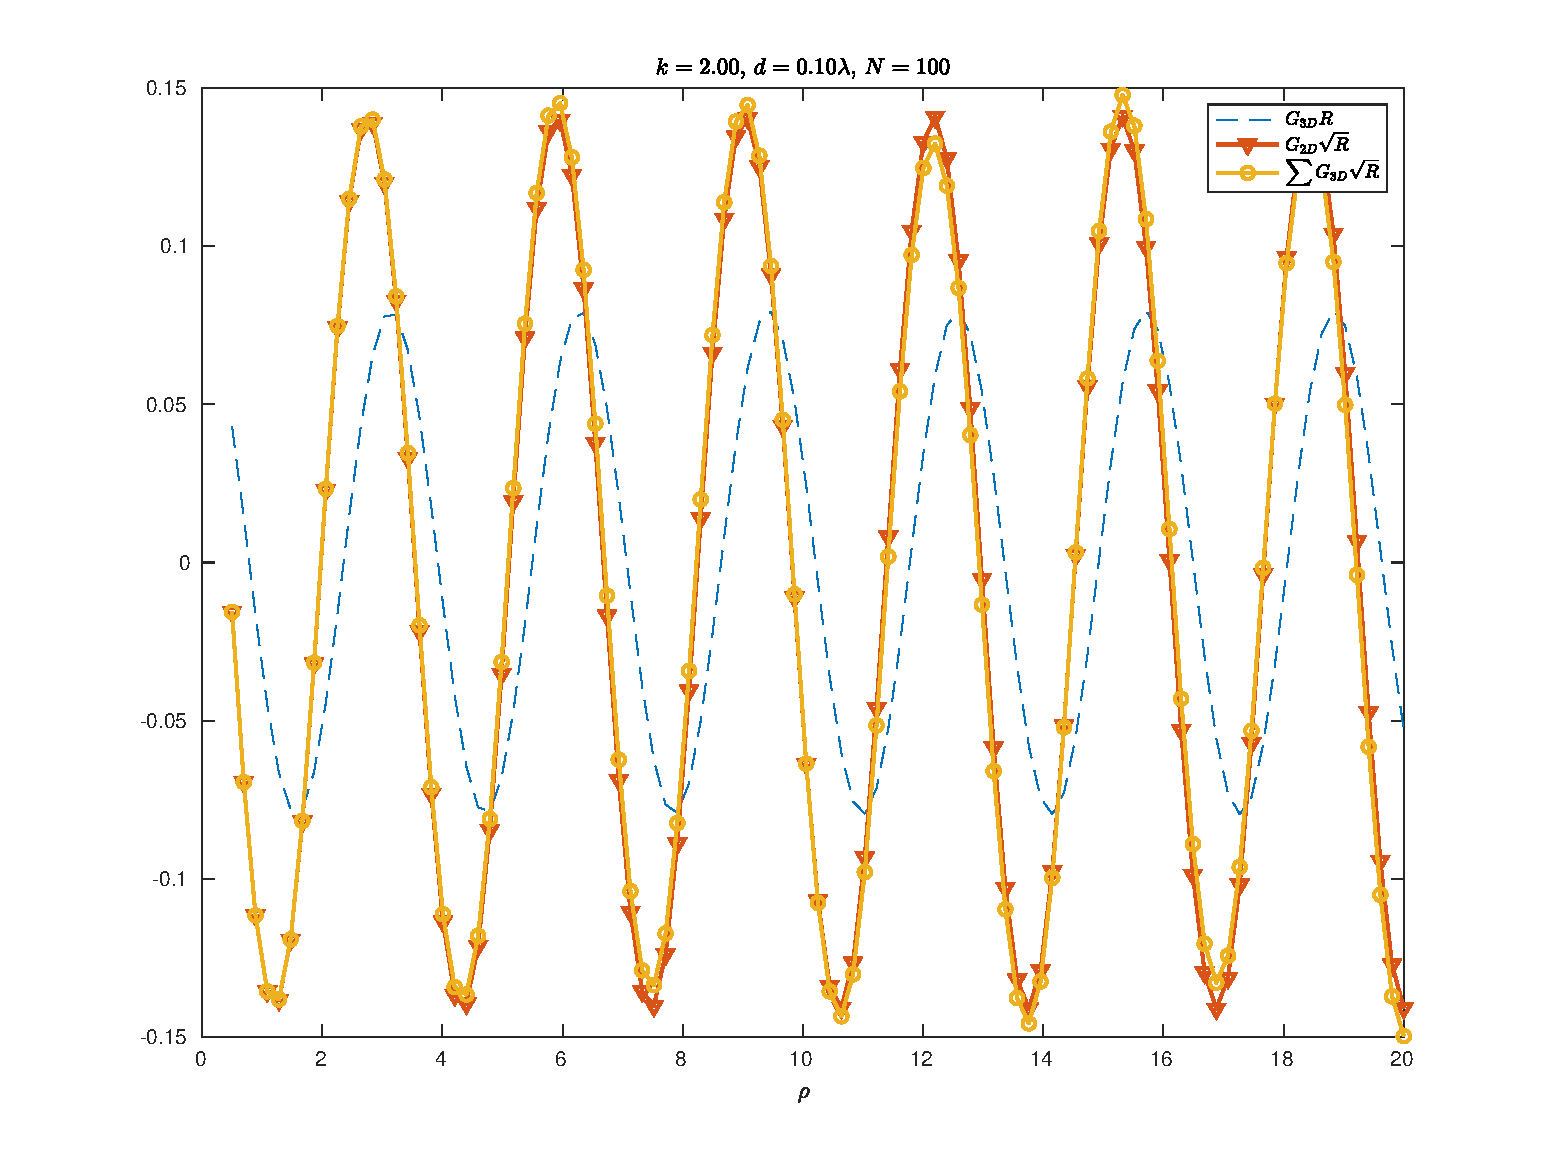
\includegraphics[width=\textwidth]{GreenFunctions_R.pdf} \\
     % \footnotesize{Green's function values as a function of $\rho$}
      \column{0.48\textwidth}
      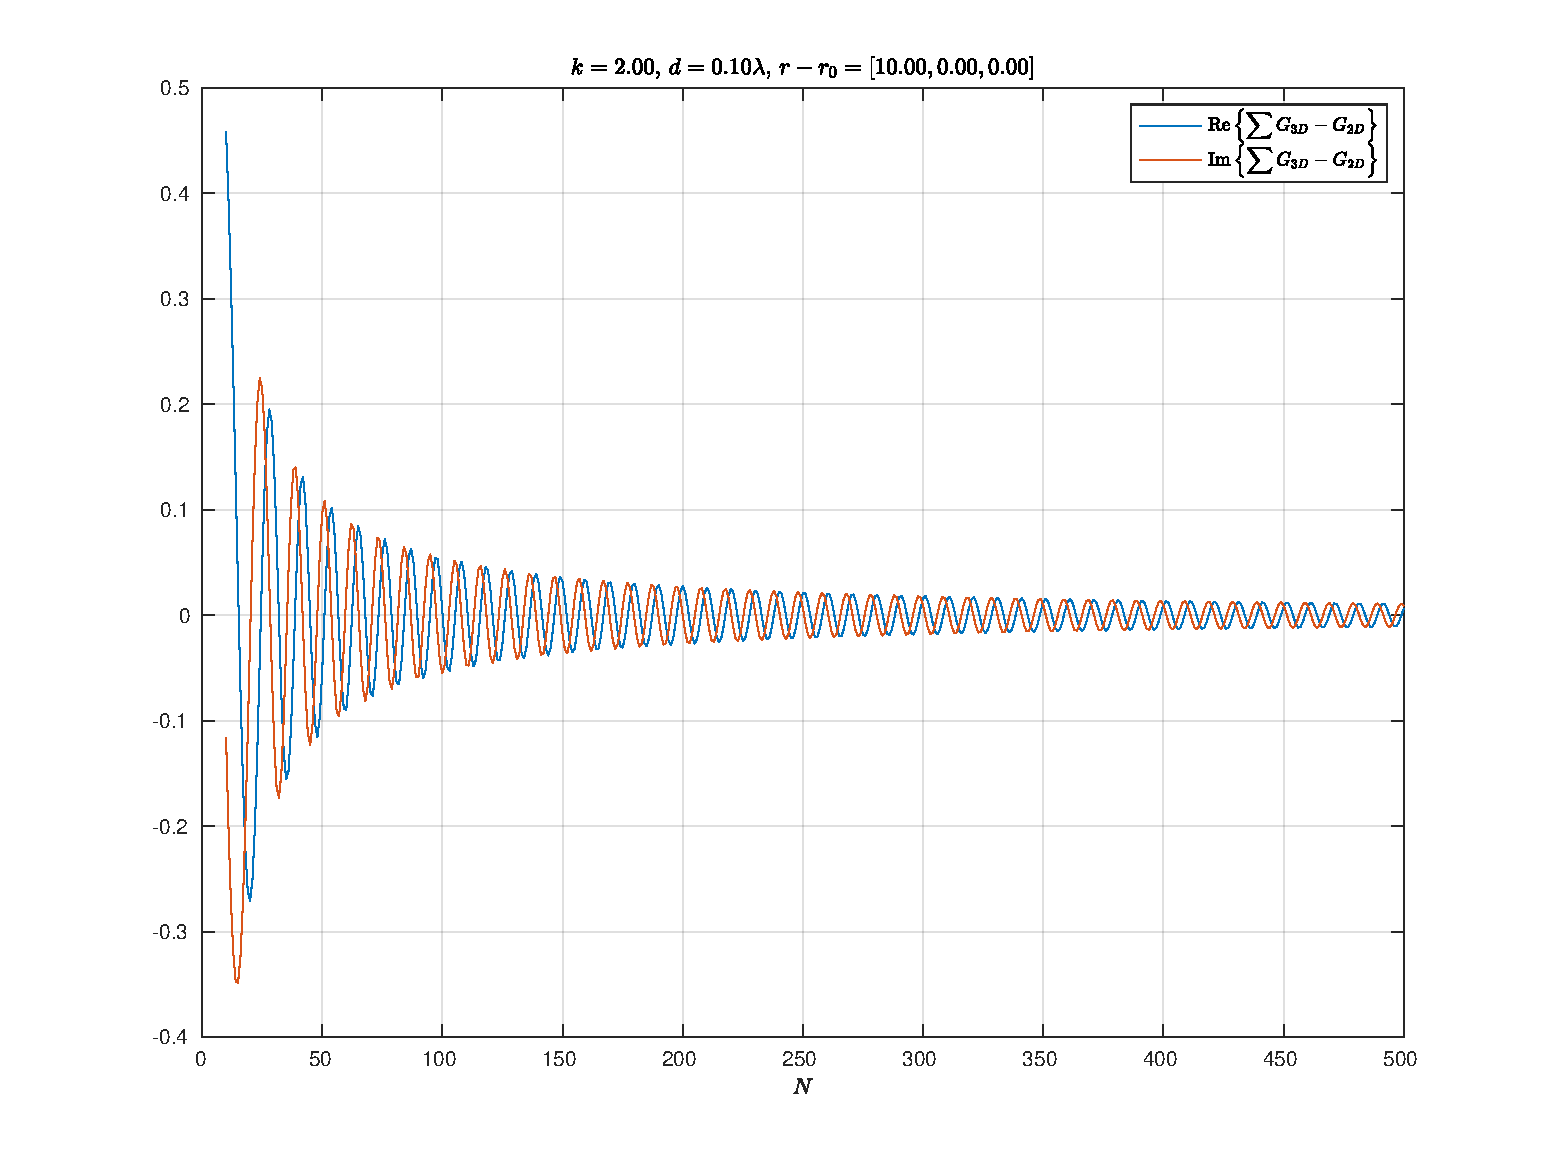
\includegraphics[width=\textwidth]{GreenFunctions_convN_reim.pdf} \\
      %\footnotesize{3D Green's function values as the number of unit
      %  cells considered (no Ewald acceleration)}
    \end{columns}
  \end{block}

  \framebreak % %%%%%%%%%%%%%%%%%%%%%%%%%%%%%%%%%%%%%%

  \begin{block}{Sanity Checks (MATLAB)}
    Equivalence of infinite sum of 3D Green's function with 2D Green's
    function on the unit cell
    \begin{columns}%[T]
      \column{0.48\textwidth}
       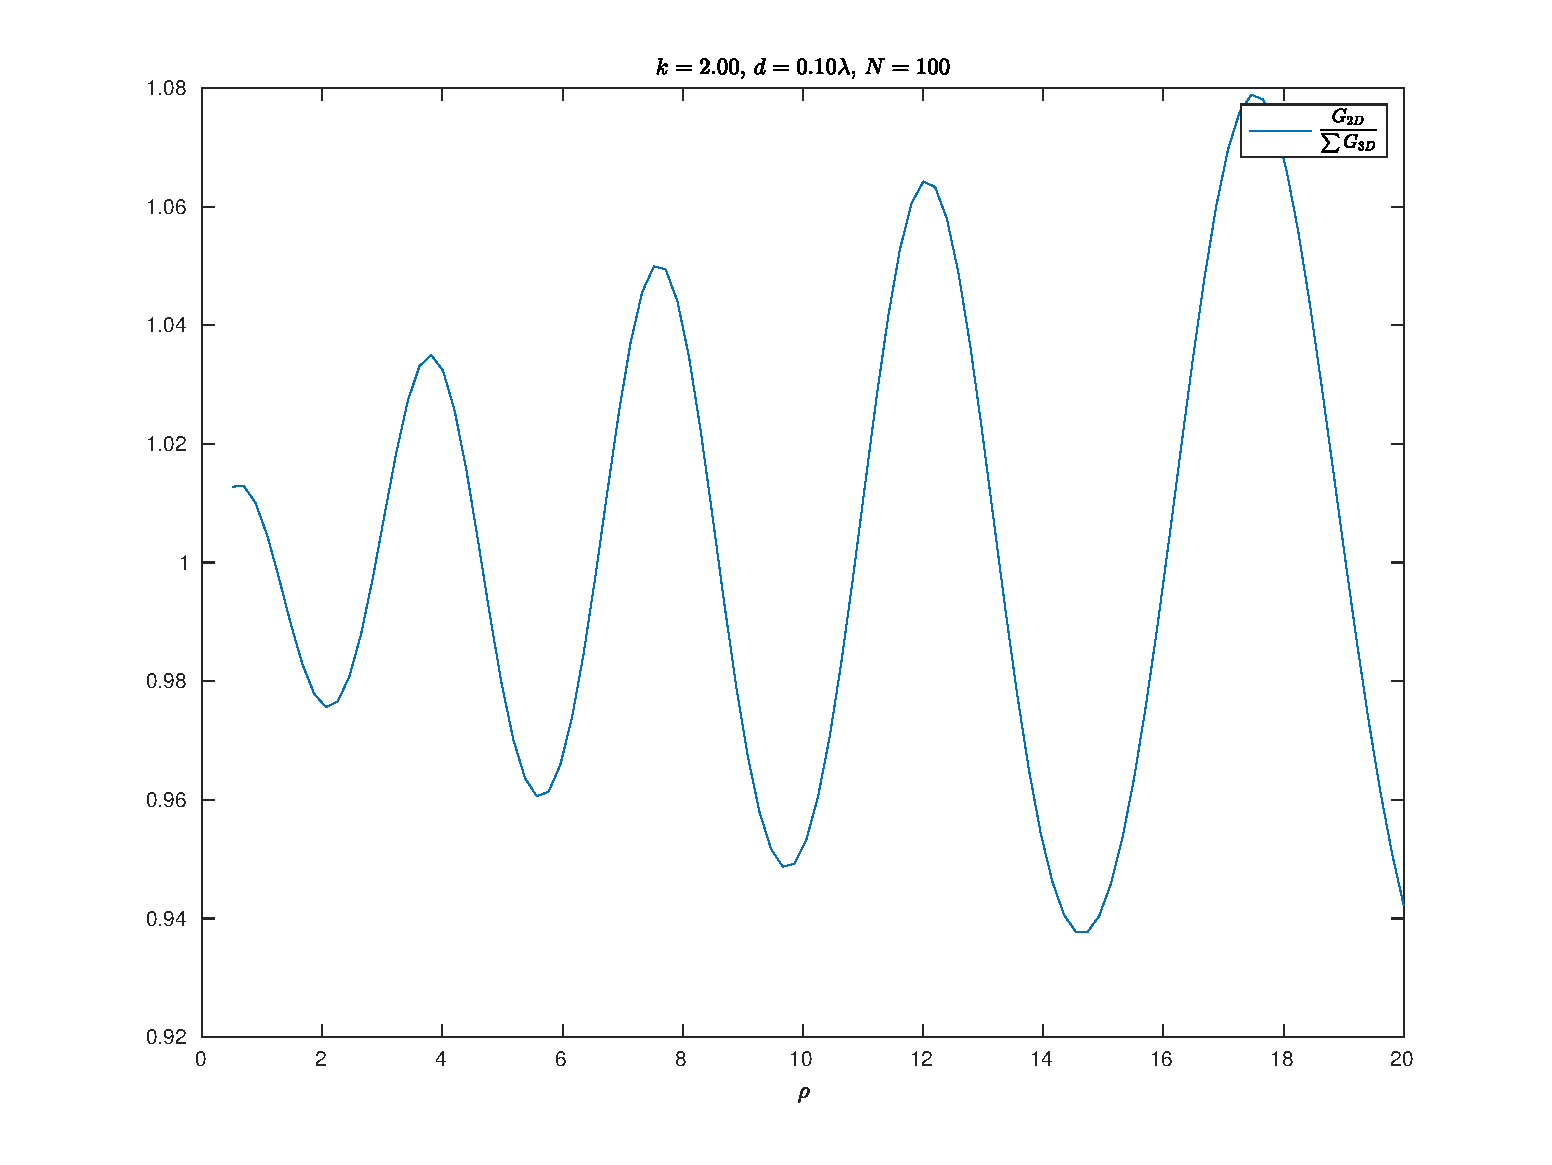
\includegraphics[width=\textwidth]{GreenFunctions_Comp.pdf} \\
%      \footnotesize{Difference Green's function values (3D summation and 2D)
%        as a function of $\rho$}
      \column{0.48\textwidth}
      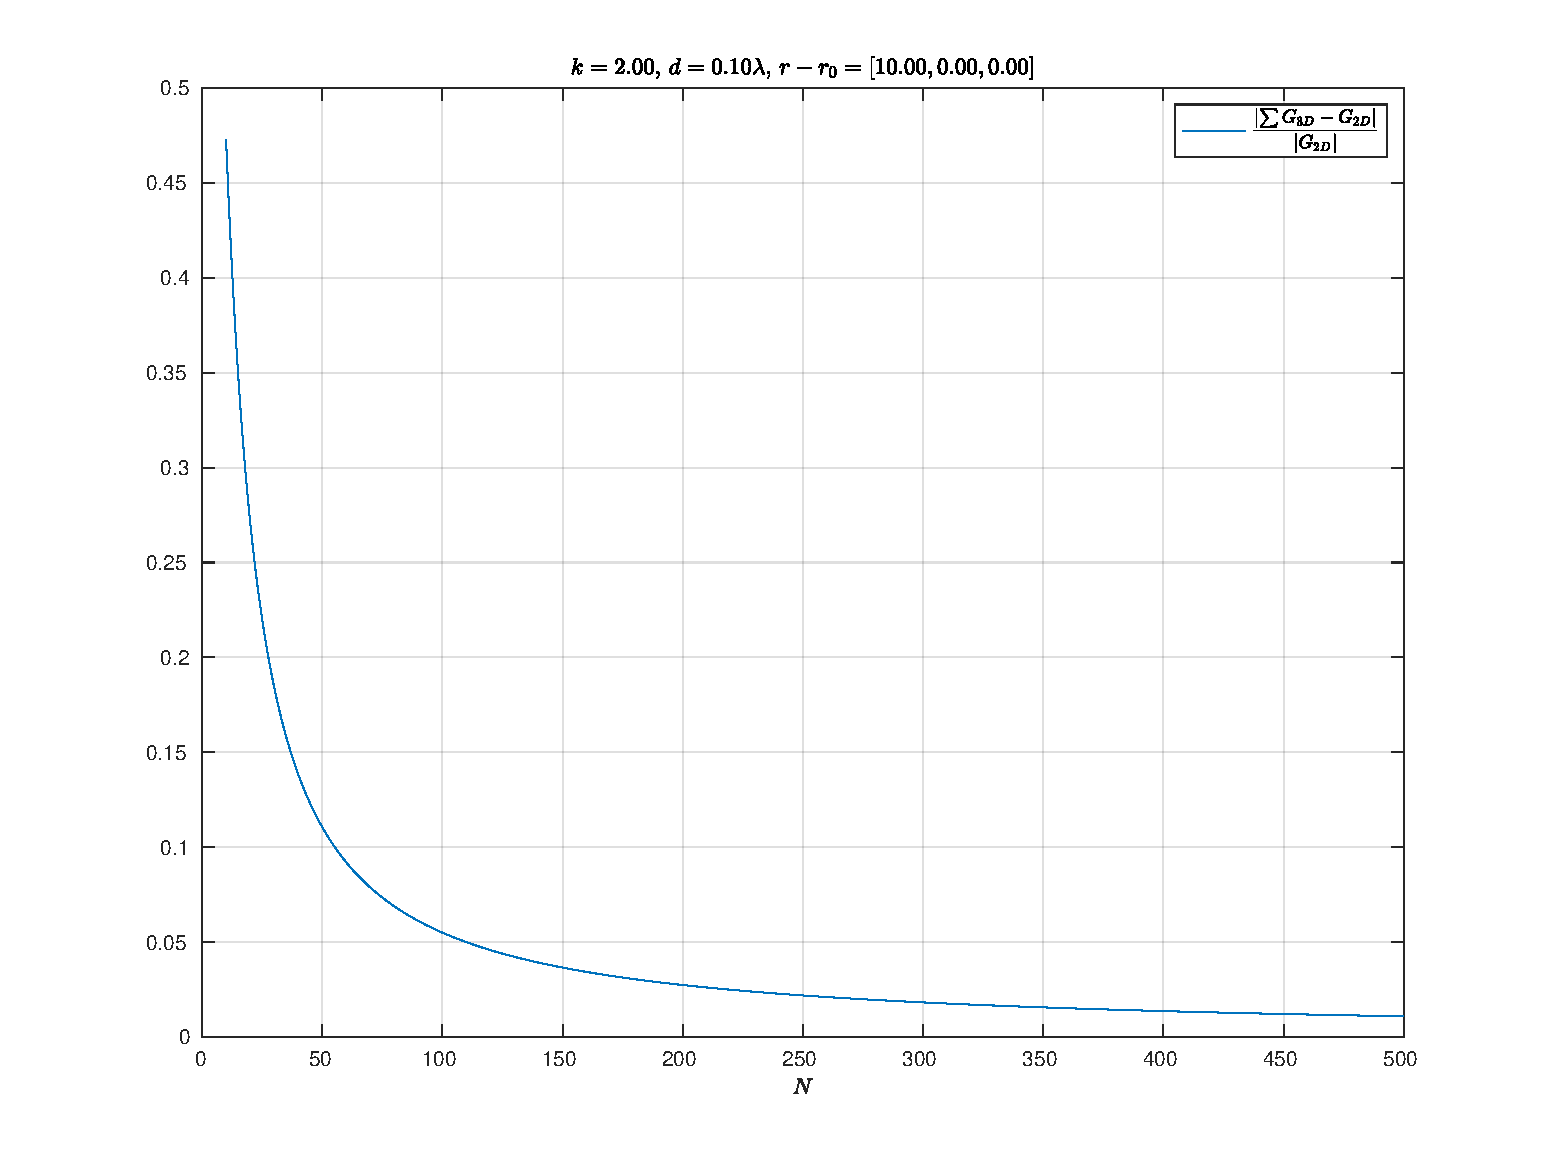
\includegraphics[width=\textwidth]{GreenFunctions_convN_abs.pdf} \\
%      \footnotesize{Difference Green's function values (3D summation
%        and 2D) with the number of unit cells (slices) considered (no
%        Ewald acceleration)}
    \end{columns}
  \end{block}

  \framebreak % %%%%%%%%%%%%%%%%%%%%%%%%%%%%%%%%%%%%%%

  \begin{block}{HOFEM Implementation}

    \begin{itemize}
    \item Coded
    \item Tested
    \end{itemize}
    
    \begin{columns}%[T]
      \column{0.45\textwidth}
      \lstinputlisting[basicstyle=\tiny,tabsize=3,frame=none,
      % caption={3D Green's Function},
      firstline=125,lastline=145]{HOFEM_output_3D_greens_function.txt}
      
      % \column{0.45\textwidth}
      % \lstinputlisting[basicstyle=\tiny,tabsize=3,frame=none,caption={2D
      %   Green's Function},firstline=125,lastline=130]{HOFEM_output_2D_greens_function.txt}
      
    \end{columns}
  \end{block}

  % \framebreak % %%%%%%%%%%%%%%%%%%%%%%%%%%%%%%%%%%%%%%

  % \lstinputlisting[basicstyle=\tiny,tabsize=3,frame=none,caption={2D
  %   Green's Function},firstline=20,lastline=30]{HOFEM_output_diff_3D_2D_greens_function_sidebyside.txt}

  \framebreak % %%%%%%%%%%%%%%%%%%%%%%%%%%%%%%%%%%%%%%

 Code output (terminal):
  
 \lstinputlisting[basicstyle=\scriptsize,tabsize=3,frame=none,
 % caption={2D Green's Function}
 ]{HOFEM_output_diff_3D_2D_greens_function_iterations.txt}


  \framebreak % %%%%%%%%%%%%%%%%%%%%%%%%%%%%%%%%%%%%%%


  \begin{columns}
    \column{0.48\textwidth} \centering
    {\includegraphics[angle=0,width=\textwidth]{Cylinder_0_5b_nearfield_3D_greens}}
    \column{0.48\textwidth} \centering
    {\includegraphics[angle=0,width=\textwidth]{Cylinder_0_5b_nearfield_3D_greens}}
  \end{columns}    

  
\end{frame}


% %%%%%%%%%%%%%%%%%%%%%%%%%%%%%%%%%%%%%%%%%%%%%%%%%%%%%%%%%%%%%%%%%%%%%%%%%
\subsection{Far Field (postprocess)}
% %%%%%%%%%%%%%%%%%%%%%%%%%%%%%%%%%%%%%%%%%%%%%%%%%%%%%%%%%%%%%%%%%%%%%%%%%

\begin{frame}[allowframebreaks]{Far Field (postprocess)}

  \begin{block}{Equivalence of Green's Functions for Far Field}
    \begin{itemize}
    \item Can we use an infinite sum of 3D Green's far-field functions
      to model the 2D Green's far-field?
      \begin{itemize}
      \item \alert {NO}
      \item and it makes sense!
      \end{itemize}
    \end{itemize}
  \end{block}
    

  \begin{block}{Far Field as Fourier Transform} 
      The Fourier Transform of a constant current contribution along
      $z$ is a delta function in the spatial frequency domain, i.e.,
      variable $\theta$:
      % 
      \begin{equation}
        \text{Far Field}(\theta,\phi) =  \alert{\delta(\theta-\pi/2)}  F(\phi)
      \end{equation}
      
    \end{block}
  
    \framebreak % %%%%%%%%%%%%%%%%%%%%%%%%%%%%%%%%%%%%%%

    \begin{columns}
      \column{0.46\textwidth} \centering
      \begin{block}{$\theta\ne 90^\circ$: \alert{Oscillations}}
        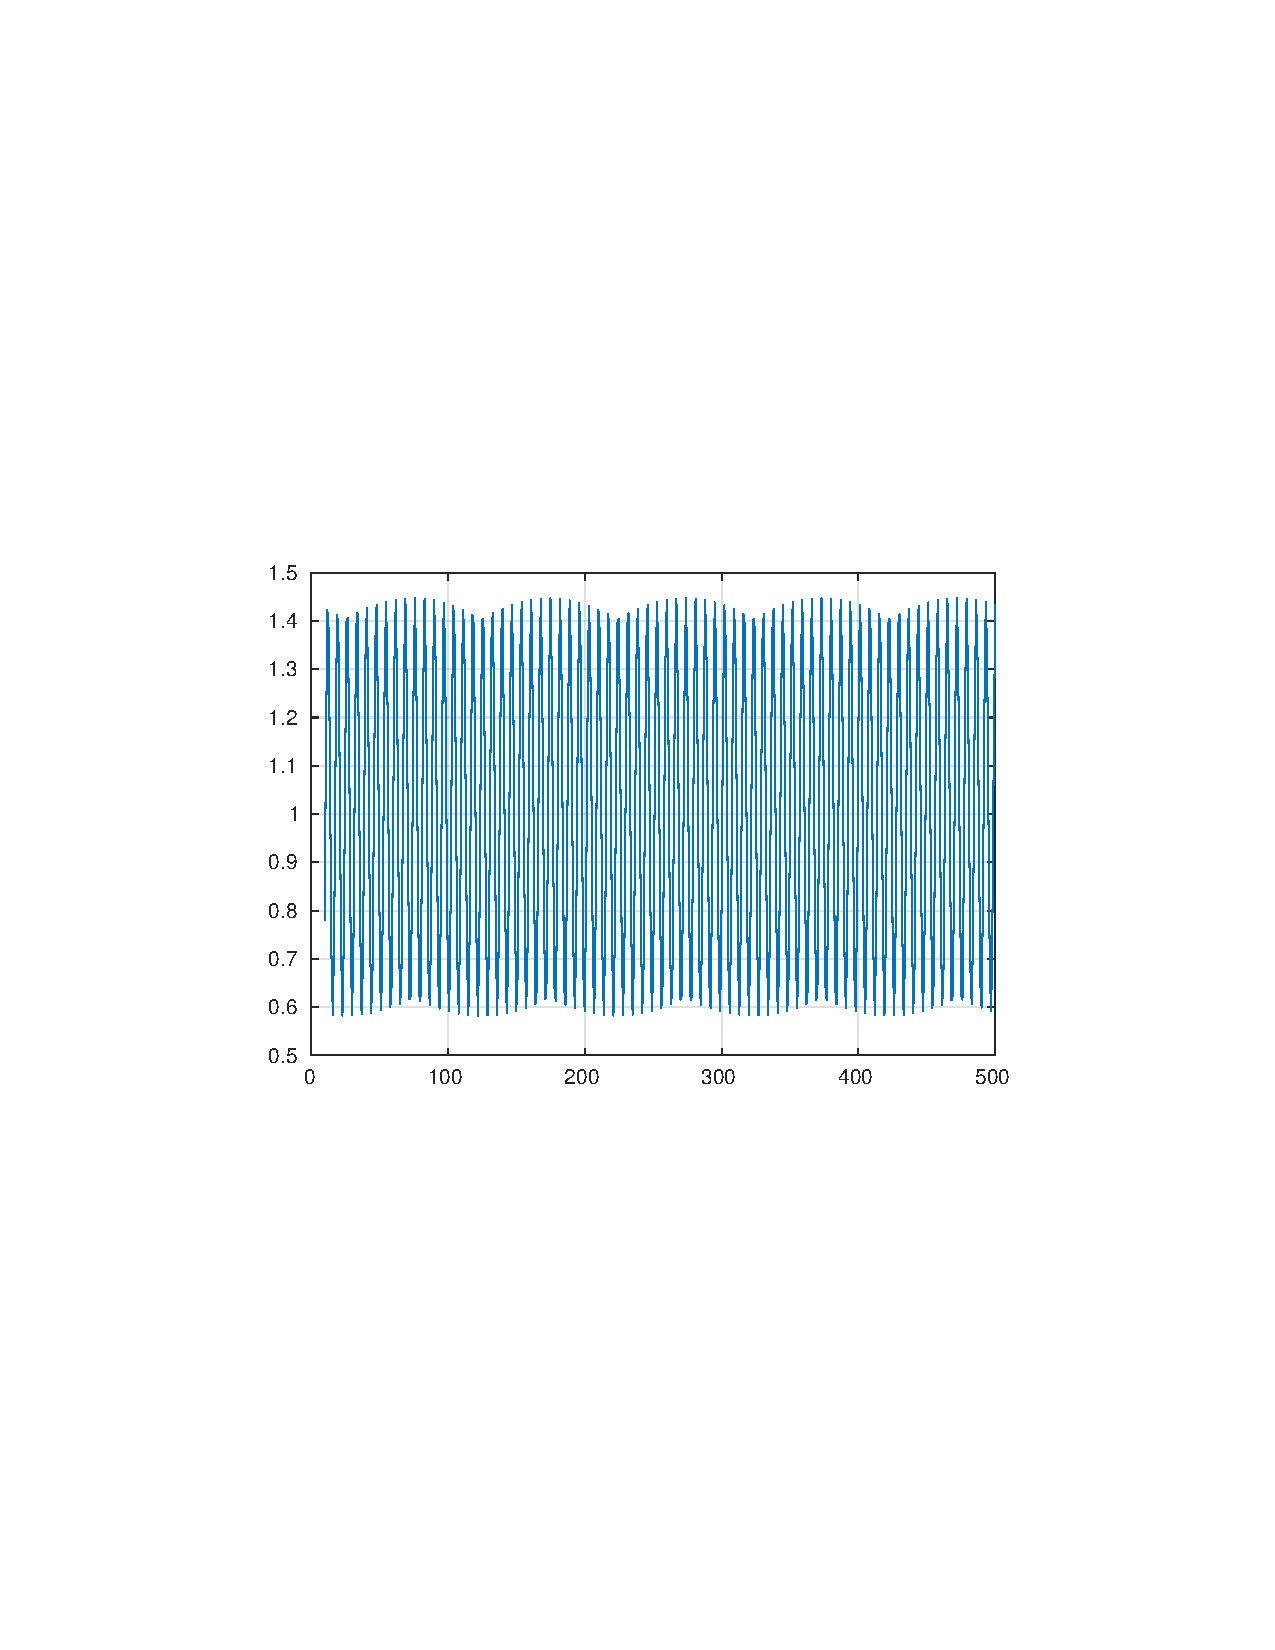
\includegraphics[clip=true,trim=100 200 100 200,width=\textwidth]{GreenFar_abs_theta45} \\
      \end{block}
      
      \column{0.46\textwidth} \centering
      \begin{block}{$\theta=90^\circ$: \alert{Divergence}}
        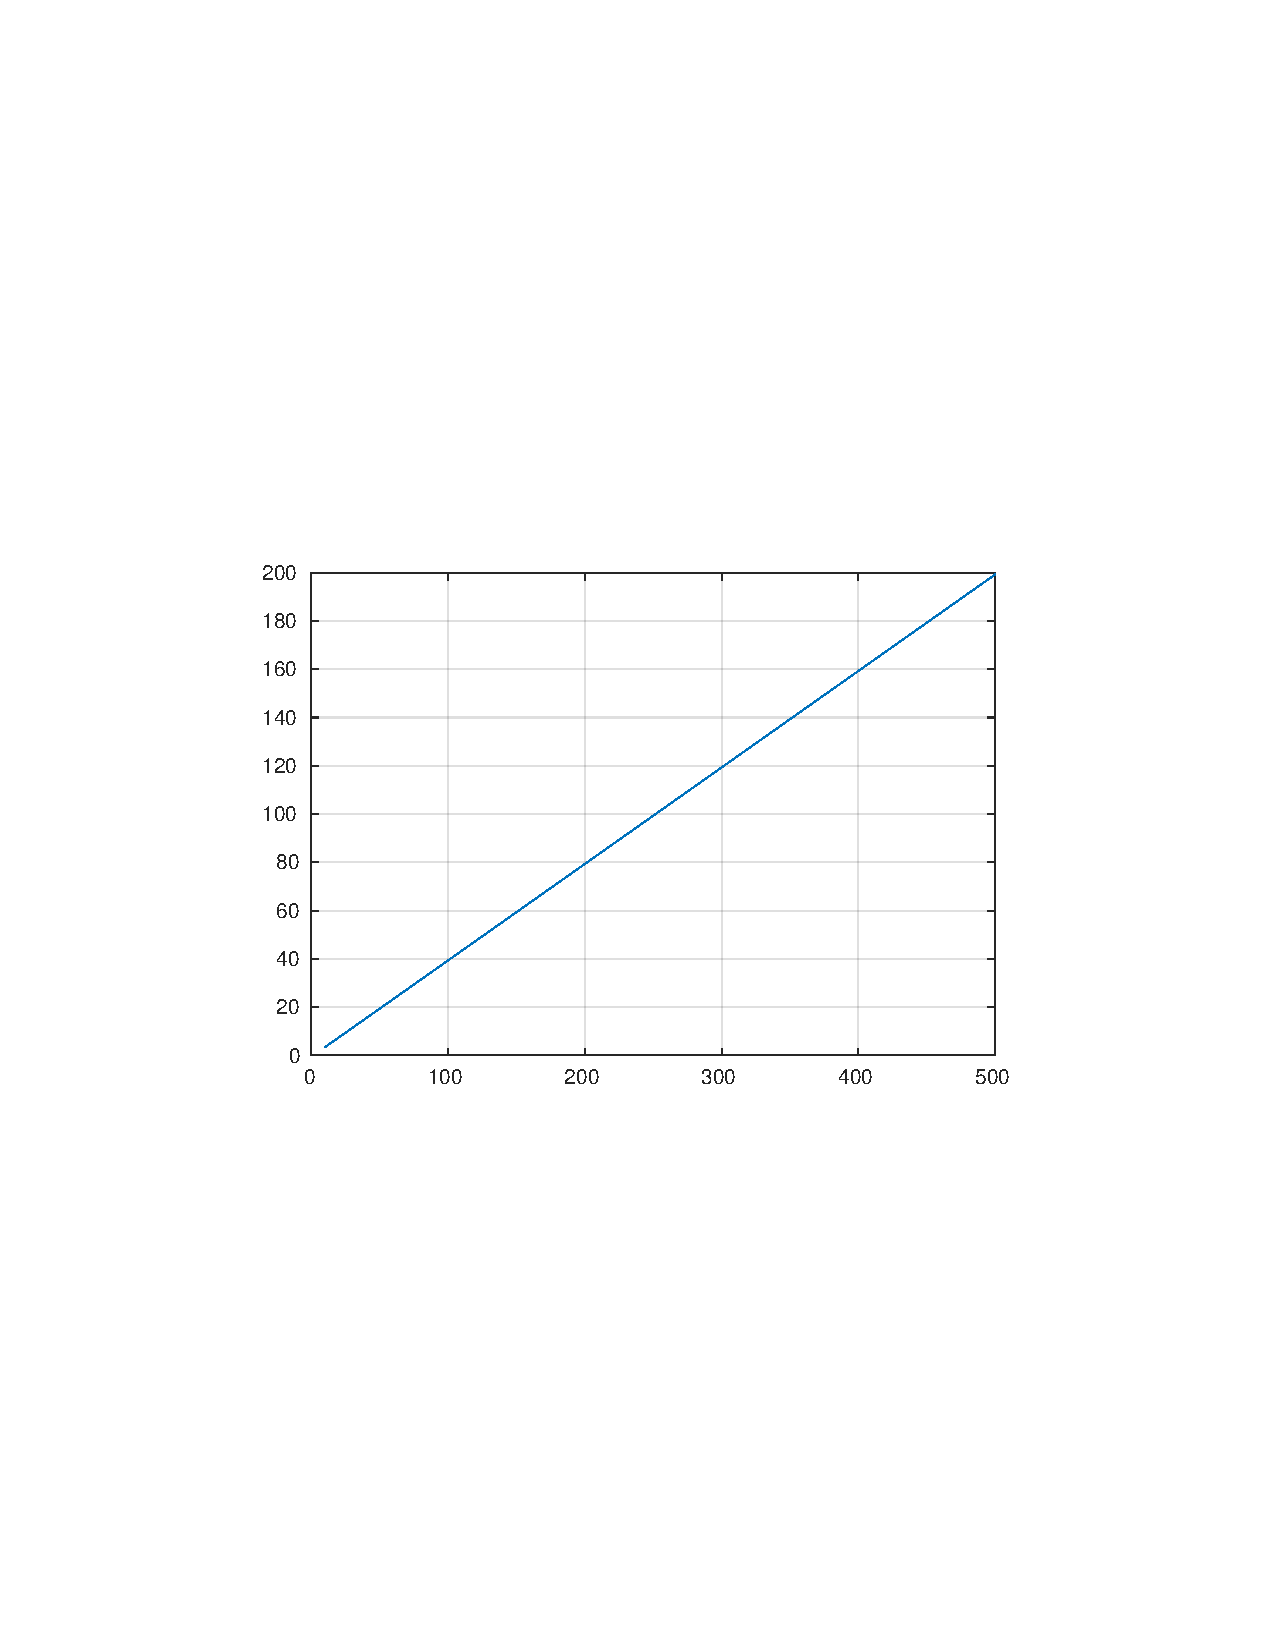
\includegraphics[clip=true,trim=100 200 100 200,width=\textwidth]{GreenFar_abs_theta90} \\
      \end{block}
            
    \end{columns}

  \end{frame}
  
  % %%%%%%%%%%%%%%%%%%%%%%%%%%%%%%%%%%%%%%%%%%%%%%%%%%%%%%%%%%%%%%%

% %%%%%%%%%%%%%%%%%%%%%%%%%%%%%%%%%%%%%%%%%%%%%%%%%%%%%%%%%%%%%%%%%%%%%%%%%
\subsection{Further Rethinking on Possible Use of  {\GreenT}}
% %%%%%%%%%%%%%%%%%%%%%%%%%%%%%%%%%%%%%%%%%%%%%%%%%%%%%%%%%%%%%%%%%%%%%%%%%

    
  \begin{frame}[plain]
    \centering    \Large{Rethinking\ldots}

    \vspace*{0.5\baselineskip}

    \centering\parbox{\textwidth}{%
      AIRBUS: \emph{\foreignlanguage{spanish}{hay un chico con nosotros que
          resuelve problemas de scattering de cilindros y no usa
          función de Hankel. Usa Green3D para calcular el campo
          (lejano) de scattering de una rodaja y \alert{le funciona.}}
        }}

      \vspace*{\baselineskip}
      
      \begin{itemize}
      \item Further study of differences between  {\GreenD} and {\GreenT}
        \begin{itemize}
        \item Obvious (after a maturation process) for far field
        \item Not so obvious for near field (i.e., in its impact in
          FE-IIEE loop)
        \end{itemize}
      \end{itemize}
      
  \end{frame}
  

% %%%%%%%%%%%%%%%%%%%%%%%%%%%%%%%%%%%%%%%%%%%%%%%%%%%%%%%%%%%%%%%

\begin{frame}[allowframebreaks]{Far Field (postprocess)}

  \begin{block}{Equivalence of Green's Functions for Far Field}
    \begin{itemize}
    \item Can we use an infinite sum of 3D Green's far-field functions
      to model the 2D Green's far-field?
      \begin{itemize}
      \item NO
      \item and it makes sense!
      \item No need of infinite sum (\alert{far field {\GreenT}/{\GreenD} is enough})
        \begin{itemize}
        \item Note that far field versions of {\GreenT} (with
          $r=\rho$) and {\GreenD} are equal up to a constant
        \end{itemize}

      \end{itemize}
    \end{itemize}
  \end{block}
    

  \begin{block}{Far Field as Fourier Transform} 
      The Fourier Transform of a constant current contribution along
      $z$ is a delta function in the spatial frequency domain, i.e.,
      variable $\theta$:
      % 
      \begin{equation}
        \text{Far Field}(\theta,\phi) =  \alert{\delta(\theta-\pi/2)}  F(\phi)
      \end{equation}
      
    \end{block}
  
    \framebreak % %%%%%%%%%%%%%%%%%%%%%%%%%%%%%%%%%%%%%%
    
    \begin{block}{{\GreenD} vs {\GreenT}}

      
      $F(\phi)$ is the same (after normalization) considering asymptotic
      expressions of {\GreenT} and {\GreenT}
      
    \begin{columns}\centering
      \column{0.4\textwidth}% \centering
      %
      \begin{equation*}
        H_0^{(2)}(k\rho)
        \enskip \overset{\rho\rightarrow\infty}{\approx} \enskip
        \sqrt{\dfrac{2 j }{\pi k \rho}} \, e^{-jk\rho}
      \end{equation*}

      \column{0.4\textwidth}% \centering
      % 
      % 
      \begin{equation*}
        \dfrac{e^{-jkR}}{4\pi R}
         \enskip \overset{r\rightarrow\infty}{\approx}  \enskip
        \dfrac{e^{-jkr}}{4\pi r} e^{j k r^\prime\! \cos\psi}
      \end{equation*}

    \end{columns}
    
    \end{block}


  \end{frame}

  
% %%%%%%%%%%%%%%%%%%%%%%%%%%%%%%%%%%%%%%%%%%%%%%%%%%%%%%%%%%%%%%%

\begin{frame}[allowframebreaks]{Near Field (FE-IIEE loop)}
  
% {\Gree3D vs {\GreenD} }


 Code output (terminal):

 \begin{itemize}
 \item From previous meeting % Large $S'-S$
   \begin{columns}%[T]
   \column{0.45\textwidth} {\GreenD} 
   \column{0.45\textwidth} {\GreenT} 
 \end{columns}   

 \lstinputlisting[basicstyle=\scriptsize,tabsize=3,frame=none,
 % caption={2D Green's Function}
 ]{HOFEM_output_diff_3D_2D_greens_function_iterations_reversed.txt}

 \vspace{\baselineskip}

 \alert{How can it work?} Note we used {\GreenT} itself (only one
 slide was considered)
 
 
 \framebreak % %%%%%%%%%%%%%%%%%%%%%%%%%%%%%%%%%%%%%%

 Code output (terminal):

 \item Large $S'-S$
   \begin{columns}[T]
   \column{0.45\textwidth} {\GreenD} 
   \column{0.45\textwidth} {\GreenT} 
 \end{columns}   

 \lstinputlisting[basicstyle=\scriptsize,tabsize=3,frame=none,
 ]{HOFEM_output_diff_3D_2D_greens_function_iterations_reversed.txt}
 
\item Small $S'-S$
   \begin{columns}%[T]
   \column{0.45\textwidth} {\GreenD} 
   \column{0.45\textwidth} {\GreenT} 
 \end{columns}   

 \lstinputlisting[basicstyle=\scriptsize,tabsize=3,frame=none,
 ]{HOFEM_output_diff_3D_2D_greens_function__small_S-Sp_iterations_reversed.txt}

 
\end{itemize}

\end{frame}

  % %%%%%%%%%%%%%%%%%%%%%%%%%%%%%%%%%%%%%%%%%%%%%%%%%%%%%%%%%%%%%%% 

% \begin{frame}[allowframebreaks]{Study of {\GreenT} vs {\GreenD}}
 
 
%   \textbf{GRAFICAS DE LAS GEOMETRIAS USADAS EN LAS PRUEBAS}


%   \begin{itemize}
%   \item Lo que le enseñamos meeting pasado fue sobre (S'-S grande,
%     espesor pequeño y S,S' rectangulares):
    
% \begin{verbatim}
% |`cylinder_05b_1`               |1      |1      |0.05     |Rectangular    |Rectangular      |1
% \end{verbatim}
    
%     \item Durante el finde (S'-S pequeño y espesor grande, con S', S circulares)
  
% \begin{verbatim}
%     |`cylinder_05e_01_01_075`       |0.1    |0.1    |1        |Circular       |Circular         |0.75
% \end{verbatim}

%     \item Para ver efecto del espesor se puede comparar 
      
% \begin{verbatim}
%     |`cylinder_05e_01_01_075`       |0.1    |0.1    |1        |Circular       |Circular         |0.75
%     |`cylinder_sp_circled_s_circled_d_1_h_005_m_075`  |0.1|0.1|0.05   |Circular    |Circular     |0.75
% \end{verbatim}

%     \item Mallado con S' sobre PEC para paranoias de J,M equivalentes.

%       Uno de los:
% \begin{verbatim}
% Espesor bajo, distancia S-S' baja:
% |`cylinder_sp_pec_s_circled_d_01_h_005_m_07`  |0  |0.1|0.05   |Circular |Circular     |0.7


% Espesor alto, distancia S-S' baja:
% |`cylinder_sp_pec_s_circled_d_01_h_1_m_07`    |0  |0.1|1      |Circular |Circular     |0.7
% \end{verbatim}

      
      
%   \end{itemize}
% \end{frame}

  % %%%%%%%%%%%%%%%%%%%%%%%%%%%%%%%%%%%%%%%%%%%%%%%%%%%%%%%%%%%%%%% 

\begin{frame}[allowframebreaks]{{\GreenD} vs {\GreenT}}{Comparison
    with analytical solution}

  \begin{itemize}
  \item Most results displayed correspond to TM and E field
  \item H field (i.e., RotE) identical conclusions
  \item By duality (satisfied by HOFEM) TE results ``should'' be
    identical (tested).
  \item Most results shown here correspond to both $S'$ and $S$
    conformal to the cylinder (circular boundary). Analogous
    results/conclusions are obtained with rectangular boundaries for
    $S'$ and $S$ (and combinations of them).
  \end{itemize}
  % \textbf{\url{cylinder_05e_01_01_075} ¿Graficas del estilo de??}

  \framebreak % %%%%%%%%%%%%%%%%%%%%%%%%%%%%

  
    \begin{columns}
        \column{0.55\textwidth}
    \includegraphics[width=\linewidth]
    {results/2D/20/300/\meshCCC{01}{1}{075}/geometry.pdf}
        \column{0.4\textwidth}
        \begin{itemize}
          \item 300\,MHz
          \item Small $S-S'$
          \item Thick slice
        \end{itemize}
    \end{columns}

    \framebreak

    Evolution scattered electric field ($S'$ over $S$)

    \vbs

    Iteration \makebox[0pt][l]{1:}\hspace{2em}
    \raisebox{\baselineskip-\height}{
      \includegraphics[width=0.3\textwidth]
      {results/2D/1/300/\meshCCC{01}{1}{075}/E_S.pdf}
      \hspace{1cm}
      \includegraphics[width=0.3\textwidth]
      {results/3D/1/300/\meshCCC{01}{1}{075}/E_S.pdf}
    }

    \vbs

    Iteration \makebox[0pt][l]{20:}\hspace{2em}
    \raisebox{\baselineskip-\height}{
      \includegraphics[width=0.3\textwidth]
      {results/2D/20/300/\meshCCC{01}{1}{075}/E_S.pdf}
      \hspace{1cm}
      \includegraphics[width=0.3\textwidth]
      {results/3D/20/300/\meshCCC{01}{1}{075}/E_S.pdf}
    }

    
    \framebreak
    Evolution scattered magnetic field ($S'$ over $S$)

    \vbs

    Iteration \makebox[0pt][l]{1:}\hspace{2em}
    \raisebox{\baselineskip-\height}{
      \includegraphics[width=0.3\textwidth]
      {results/2D/1/300/\meshCCC{01}{1}{075}/H_S.pdf}
      \hspace{1cm}
      \includegraphics[width=0.3\textwidth]
      {results/3D/1/300/\meshCCC{01}{1}{075}/H_S.pdf}
    }

    \vbs

    Iteration \makebox[0pt][l]{20:}\hspace{2em}
    \raisebox{\baselineskip-\height}{
      \includegraphics[width=0.3\textwidth]
      {results/2D/20/300/\meshCCC{01}{1}{075}/H_S.pdf}
      \hspace{1cm}
      \includegraphics[width=0.3\textwidth]
      {results/3D/20/300/\meshCCC{01}{1}{075}/H_S.pdf}
    }


    \framebreak

    Evolution electric field on $S'$

    \vbs

    Iteration \makebox[0pt][l]{1:}\hspace{2em}
    \raisebox{\baselineskip-\height}{
      \includegraphics[width=0.3\textwidth]
      {results/2D/1/300/\meshCCC{01}{1}{075}/E_Sp.pdf}
      \hspace{1cm}
      \includegraphics[width=0.3\textwidth]
      {results/3D/1/300/\meshCCC{01}{1}{075}/E_Sp.pdf}
    }

    \vbs

    Iteration \makebox[0pt][l]{20:}\hspace{2em}
    \raisebox{\baselineskip-\height}{
      \includegraphics[width=0.3\textwidth]
      {results/2D/20/300/\meshCCC{01}{1}{075}/E_Sp.pdf}
      \hspace{1cm}
      \includegraphics[width=0.3\textwidth]
      {results/3D/20/300/\meshCCC{01}{1}{075}/E_Sp.pdf}
    }

    \framebreak

    \begin{itemize}
    \item Higher error with {\GreenT}
      \begin{itemize}
      \item This is a case with small distance $S-S'$ and large thickness
      \item Nevertheless, the error is always significantly higher
        than {\GreenD}
      \end{itemize}
    \item {\GreenT} does not converge to right solution
    \item Components $E_x$, $E_z$, $H_y$ are not null \\
      \footnotesize{(issue of \alert{($\ast$)} certainly added confusion on the
      debugging/verification of the code)}
      \begin{itemize}
      \item Much higher levels with {\GreenT}
      \item {\GreenT} (the Green's function itself) generates non null
        $E_x$, $E_z$, $H_y$ from $E_z$ on $S'$
      \item {\GreenD} (the Green's function itself) does not generate
        any $E_x$, $E_z$, $H_y$
        \begin{itemize}
        \item Numerically, non-zero levels of $E_x$, $E_z$, $H_y$ are
          generated because numerical FEM solution has non zero levels of
          $E_x$, $E_z$, $H_y$ (tested!)
        \end{itemize}
      \end{itemize}
    \item Numerical noise always present  due to discretization 
      \begin{itemize}
      \item Clearly visible in this case
      \item Decreases with finer discretization ---FEM mesh--- (tested!)
      \end{itemize}
    \end{itemize}
    
    {\footnotesize \alert{($\ast$)} Issue of GiD/HOFEM-GUI representation of fields on surface}
  
\end{frame}

% %%%%%%%%%%%%%%%%%%%%%%%%%%%%%%%%%%%%%%%%%%%%%%%%%%%%%%%%%%%%%%%

% Esto es un tema que no esta relacionado directamente con 2D
% Emulation sino genral del código pero se lo cuento aqui a Airbus
% porque viene a cuento.

% %%%%%%%%%%%%%%%%%%%%%%%%%%%%%%%%%%%%%%%%%%%%%%%%%%%%%%%%%%%%%%%%%%%%%%%%%
\subsection{A note on Field Representation on Surfaces}
% %%%%%%%%%%%%%%%%%%%%%%%%%%%%%%%%%%%%%%%%%%%%%%%%%%%%%%%%%%%%%%%%%%%%%%%%%

\begin{frame}[plain]
  \centering    \Large{Rethinking\ldots}
  
  {\footnotesize \alert{($\ast$)} Issue of GiD/HOFEM-GUI representation of fields on surface}
  
\end{frame}

% %%%%%
  
\begin{frame}[allowframebreaks]{GiD/HOFEM-GUI Field Representation 
    on Surfaces}{Examples with PEC surfaces}

  \begin{itemize}
  \item $E_z$ should be null on the  caps (top and
    bottom $y=\text{cte}$)

    \vbs
   
    \begin{columns}%[T]
      \centering
      \column{0.48\textwidth}\centering
      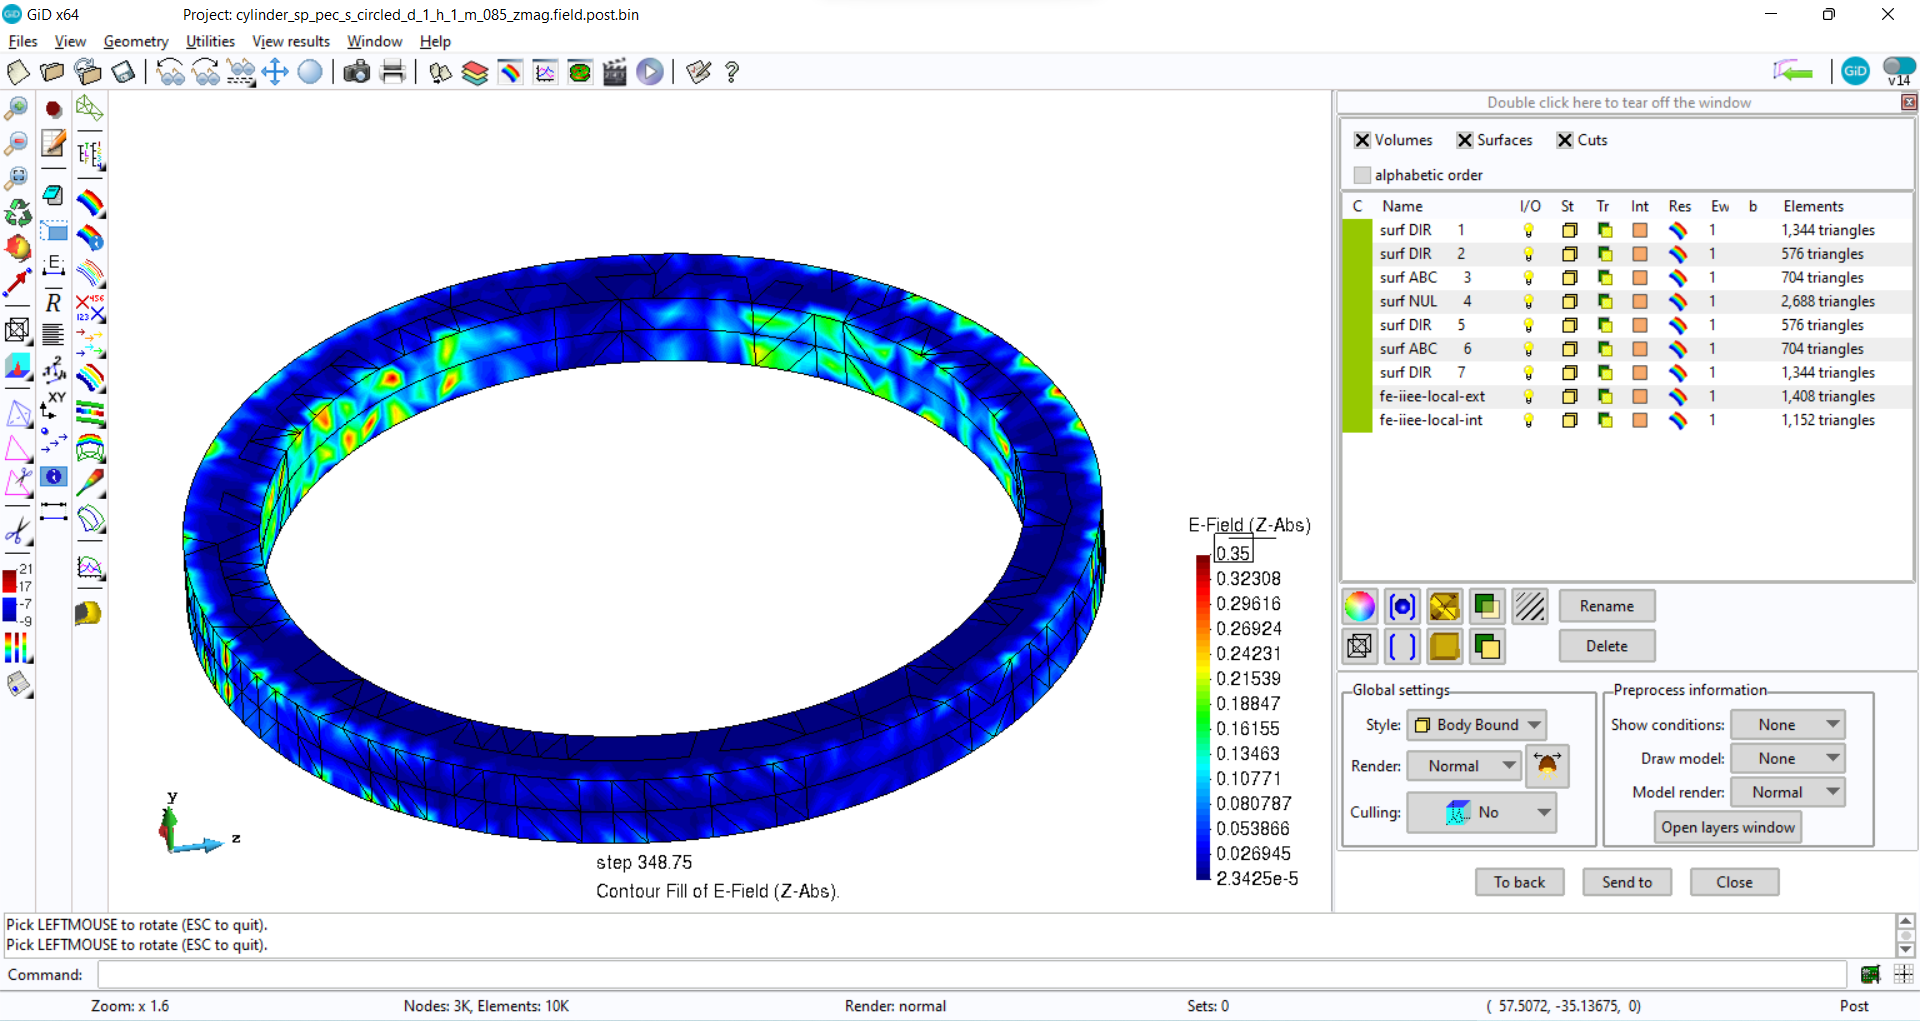
\includegraphics[width=\textwidth,clip=true,trim=70 0 350 140]
      {Ez_original} \\
      \footnotesize{$\abs{E_z}$ (default color scale)}
      \column{0.48\textwidth}\centering
      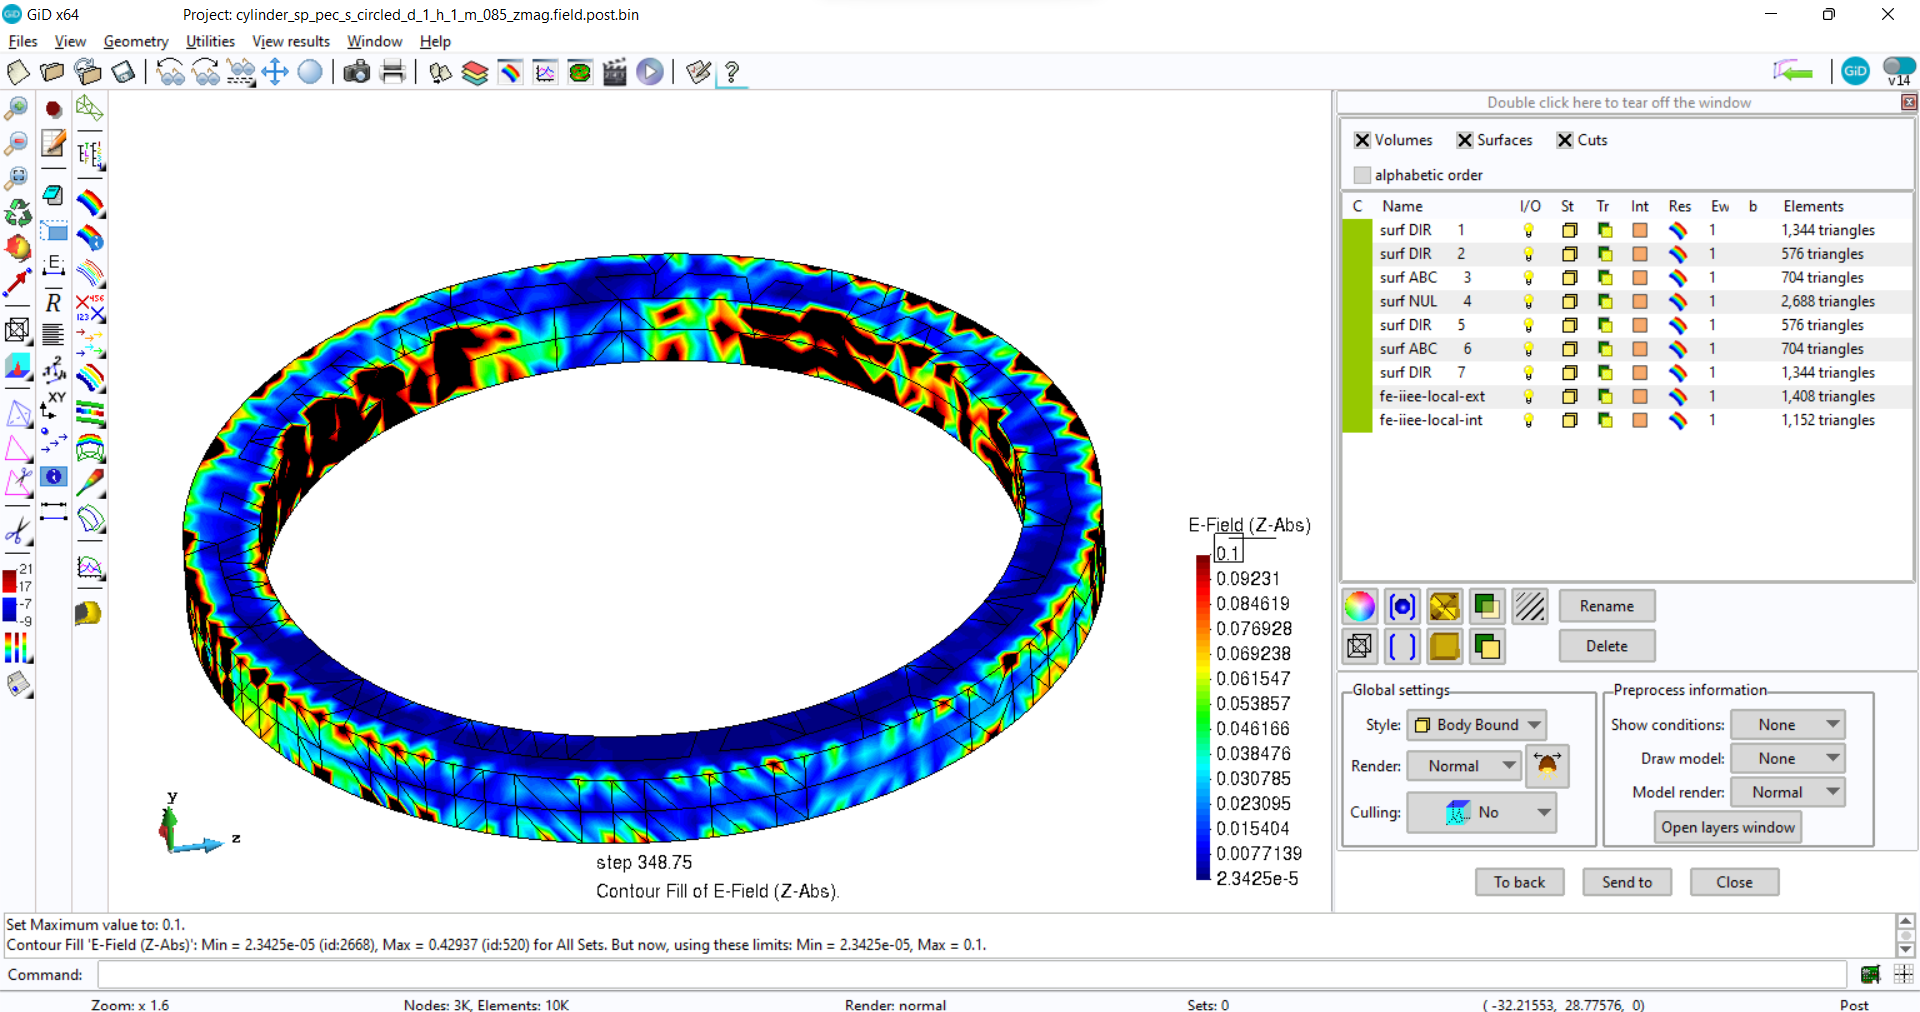
\includegraphics[width=\textwidth,clip=true,trim=70 0 350 140]
      {Ez_original_saturado_01} \\
      \footnotesize{$\abs{E_z}$ (saturated color scale)}
    \end{columns}
    

    \framebreak % %%%%%%%%%%%%%

  \item $E_y$ should be null on the cylinder ``sides'' (i.e., on the
    PEC cylinder)

    \vbss
   
    \begin{center}
     \begin{columns}%[T]
%      \column{0.48\textwidth}\centering
      % \includegraphics[width=\textwidth,clip=true,trim=70 0 350 140]
      % {Ey_original} \\
      % \footnotesize{$\abs{E_y}$ }
      \column{0.70\textwidth}\centering
      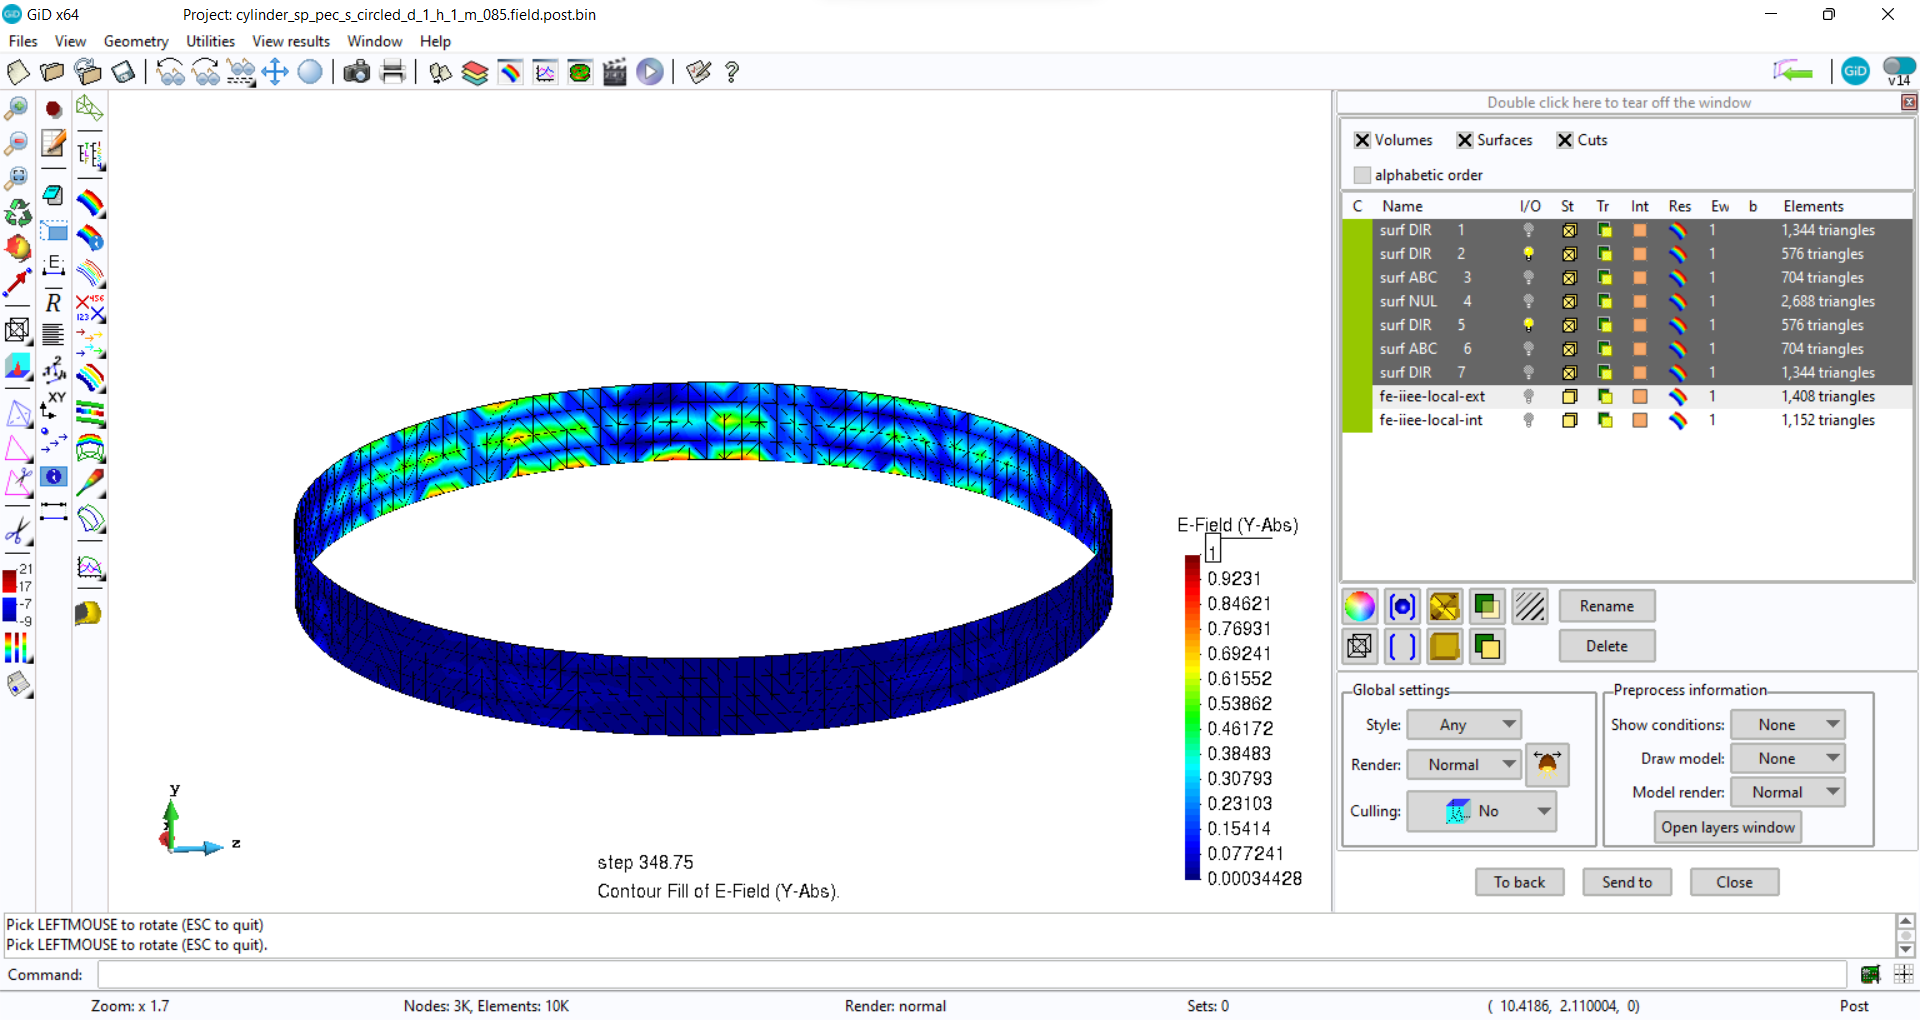
\includegraphics[width=\textwidth,clip=true,trim=70 0 350 140]
      {Ey_internal_cylinder} \\
      \footnotesize{$\abs{E_y}$ (only PEC cylinder surface shown)}
    \end{columns}
  \end{center}
  \end{itemize}
\end{frame}

% %%%%%%%%%%%%%%%%%%%%%%%%%%%%%%%%%%%%%%%%%%%%%%%%%%%%%%%%%%%%%%%

\begin{comment} % NO ES MUY CLARA LA CONCLUSION (por tema de como sale la Green3D o el campo  H) ASI QUE SE OMITEN

\begin{frame}[allowframebreaks]{Effect of Discretization}{Simple test
    changing frequency \alert{(note other electrical distances also
      change)}}


%    $300\,\text{MHz}$ \makebox[0pt][l]{20:}\hspace{2em}
    \raisebox{\baselineskip-\height}{
      \includegraphics[width=0.3\textwidth]
      {results/2D/20/300/\meshCCC{01}{1}{075}/E_S.pdf}
      \hspace{1cm}
      \includegraphics[width=0.3\textwidth]
      {results/2D/20/300/\meshCCC{01}{1}{075}/H_S.pdf}
    }

    
    \vbs

%    Lower frequency \makebox[0pt][l]{1:}\hspace{2em}
    \raisebox{\baselineskip-\height}{
      \includegraphics[width=0.3\textwidth]
      {results/2D/20/30/\meshCCC{01}{1}{075}/E_S.pdf}
      \hspace{1cm}
      \includegraphics[width=0.3\textwidth]
      {results/2D/20/30/\meshCCC{01}{1}{075}/H_S.pdf}
    }

  \end{frame}
  
\end{comment} % %%%%%%%%%%%
  
  % %%%%%%%%%%%%%%%%%%%%%%%%%%%%%%%%%%%%%%%%%%%%%%%%%%%%%%%%%%%%%%% 

\begin{comment} % NO ES MUY CLARA LA CONCLUSION (la quitamos)

\begin{frame}[allowframebreaks]{Effect of Distance $S'-S$}{Scattered near field}

    \begin{columns}
      \column{0.25\textwidth}
        \includegraphics[width=\linewidth]
        {results/2D/20/300/\meshCCC{01}{1}{075}/geometry.pdf}

        \includegraphics[width=\linewidth]
        {results/2D/20/300/\meshCCC{1}{1}{075}/geometry.pdf}
      \column{0.3\textwidth}
        
        \includegraphics[width=\linewidth]
        {results/2D/20/300/\meshCCC{01}{1}{075}/E_S.pdf}
        
        \includegraphics[width=\linewidth]
        {results/2D/20/300/\meshCCC{1}{1}{075}/E_S.pdf}

      
    \column{0.3\textwidth}
      \hfill\GreenT\hfill\mbox{}

        \includegraphics[width=\linewidth]
        {results/3D/20/300/\meshCCC{01}{1}{075}/E_S.pdf}
        
        \includegraphics[width=\linewidth]
        {results/3D/20/300/\meshCCC{1}{1}{075}/E_S.pdf}
        

    \end{columns}

    \begin{itemize}
    \item  {\GreenT} results always worse than {\GreenD}
    \item Difficult comparison ($S$ is not at the same electrical distance) 
    \end{itemize}
    
  \end{frame}

\end{comment}  % %%%%%

  % %%%%%%%%%%%%%%%%%%%%%%%%%%%%%%%%%%%%%%%%%%%%%%%%%%%%%%%%%%%%%%% 

\begin{comment} % Idem que anterior

  \begin{frame}[allowframebreaks]{Effect of Distance $S'-S$}{FEM solution}

    \begin{columns}
      \column{0.25\textwidth}

        \includegraphics[width=\linewidth]
        {results/2D/20/300/\meshCCC{01}{1}{075}/geometry.pdf}

        \includegraphics[width=\linewidth]
        {results/2D/20/300/\meshCCC{1}{1}{075}/geometry.pdf}
      \column{0.3\textwidth}
      \hfill\GreenD\hfill\mbox{}
        
        \includegraphics[width=\linewidth]
        {results/2D/20/300/\meshCCC{01}{1}{075}/E_Sp.pdf}
        
        \includegraphics[width=\linewidth]
        {results/2D/20/300/\meshCCC{1}{1}{075}/E_Sp.pdf}

      
    \column{0.3\textwidth}
      \hfill\GreenT\hfill\mbox{}

        \includegraphics[width=\linewidth]
        {results/3D/20/300/\meshCCC{01}{1}{075}/E_Sp.pdf}
        
        \includegraphics[width=\linewidth]
        {results/3D/20/300/\meshCCC{1}{1}{075}/E_Sp.pdf}
        

    \end{columns}

    \begin{itemize}
      \item The IIEE iterative method has low effect when $S-S'$ is larger.
    \end{itemize}
    
  \end{frame}
  
\end{comment}  % %%%%%
  
  % %%%%%%%%%%%%%%%%%%%%%%%%%%%%%%%%%%%%%%%%%%%%%%%%%%%%%%%%%%%%%%% 
  
\begin{frame}[allowframebreaks]{Effect of ``Thickness''}{Scattered
    near field ---\alert{Note error in figure captions: thickness is
      $0.05\,\lambda$ for the thin slice---}}
    
    \begin{columns}
      \column{0.25\textwidth}
        \includegraphics[width=\linewidth]
        {results/2D/20/300/\meshCCC{01}{1}{075}/geometry.pdf}

        \includegraphics[width=\linewidth]
        {results/2D/20/300/\meshCCC{01}{005}{075}/geometry.pdf}
      \column{0.3\textwidth}
      \hfill\GreenD\hfill\mbox{}
        
        \includegraphics[width=\linewidth]
        {results/2D/20/300/\meshCCC{01}{1}{075}/E_S.pdf}
        
        \includegraphics[width=\linewidth]
        {results/2D/20/300/\meshCCC{01}{005}{075}/E_S.pdf}

      
    \column{0.3\textwidth}
      \hfill\GreenT\hfill\mbox{}

        \includegraphics[width=\linewidth]
        {results/3D/20/300/\meshCCC{01}{1}{075}/E_S.pdf}
        
        \includegraphics[width=\linewidth]
        {results/3D/20/300/\meshCCC{01}{005}{075}/E_S.pdf}
        

    \end{columns}

  \end{frame}

  \begin{frame}[allowframebreaks]{Effect of ``Thickness''}{FEM solution
    ---\alert{Note error in figure captions: thickness is
      $0.05\,\lambda$ for the thin slice---}}
    
    \begin{columns}
      \column{0.25\textwidth}
        \includegraphics[width=\linewidth]
        {results/2D/20/300/\meshCCC{01}{1}{075}/geometry.pdf}

        \includegraphics[width=\linewidth]
        {results/2D/20/300/\meshCCC{01}{005}{075}/geometry.pdf}
      \column{0.3\textwidth}
      \hfill\GreenD\hfill\mbox{}
        
        \includegraphics[width=\linewidth]
        {results/2D/20/300/\meshCCC{01}{1}{075}/E_Sp.pdf}
        
        \includegraphics[width=\linewidth]
        {results/2D/20/300/\meshCCC{01}{005}{075}/E_Sp.pdf}

      
    \column{0.3\textwidth}
      \hfill\GreenT\hfill\mbox{}

        \includegraphics[width=\linewidth]
        {results/3D/20/300/\meshCCC{01}{1}{075}/E_Sp.pdf}
        
        \includegraphics[width=\linewidth]
        {results/3D/20/300/\meshCCC{01}{005}{075}/E_Sp.pdf}
        

    \end{columns}

    \framebreak 
    
    \begin{itemize}
    \item The thickness is the main factor for error with {\GreenT}
    \item {\GreenD} behaves great!
    \item Always lower error  with thin slices% (although convergence is slow)
    \end{itemize}
    
    
  \end{frame}

    

  % %%%%%%%%%%%%%%%%%%%%%%%%%%%%%%%%%%%%%%%%%%%%%%%%%%%%%%%%%%%%%%% 
  

  \begin{comment} %%%%%%%  POR HACER
    
  \begin{frame}[allowframebreaks]{Effect on Polarization Purity}

    \begin{itemize}
    \item With ``thickness'' \textbf{Usamos espesor gordo para que se
        note:} Por ejemplo, O bien
      \url{cylinder_sp_circled_s_circled_d_1_h_1_m_075} o bien
      \url{cylinder_sp_circled_s_circled_d_01_h_1_m_075} (no se en
      cual se notará mas según distancia S'-S, uhm.....)

      \vskip 1em
      
      \begin{columns}%[T]
      \column{0.48\textwidth}
      \FIGURA{\GreenT}
%      \includegraphics[width=\textwidth]{kk_iter1} \\
%      \footnotesize{kkkkk}
      \column{0.48\textwidth}
      \FIGURA{\GreenD}
%      \includegraphics[width=\textwidth]{kk_iter82} \\
      %\footnotesize{kkkk}
    \end{columns}
  \end{itemize}
    \begin{itemize}
    \item Conclusion 1
    \item \ldots
    \end{itemize}
    
  \end{frame}

  \end{comment} %%%%%%%%
  
  % %%%%%%%%%%%%%%%%%%%%%%%%%%%%%%%%%%%%%%%%%%%%%%%%%%%%%%%%%%%%%%% 
  
  \begin{frame}[allowframebreaks]{Other Effects (paranoic
      mode)}{Effect of $S'$ on PEC cylinder}

    \begin{columns}
    \column{0.25\textwidth}

        \includegraphics[width=\linewidth]
        {results/3D/20/300/\meshCCC{1}{1}{075}/geometry.pdf}
        
        \includegraphics[width=\linewidth]
        {results/3D/20/300/\meshPC{1}{1}{085}/geometry.pdf}
      \column{0.3\textwidth}

        \includegraphics[width=\linewidth]
        {results/2D/20/300/\meshCCC{1}{1}{075}/E_S.pdf}

        \includegraphics[width=\linewidth]
        {results/2D/20/300/\meshPC{1}{1}{085}/E_S.pdf}
      \column{0.3\textwidth}
        
        \includegraphics[width=\linewidth]
        {results/2D/20/300/\meshCCC{1}{1}{075}/H_S.pdf}
        
        \includegraphics[width=\linewidth]
        {results/2D/20/300/\meshPC{1}{1}{085}/H_S.pdf}

    \end{columns}
    
  \end{frame}


  % %%%%%%%%%%%%%%%%%%%%%%%%%%%%%%%%%%%%%%%%%%%%%%%%%%%%%%%%%%%%%%% 
  
  \begin{frame}[allowframebreaks]{Other Effects (paranoic
      mode)}{Effect of $S'$, $S$ Curved}
    
      \begin{columns}
    \column{0.25\textwidth}

        \includegraphics[width=\linewidth]
        {results/3D/20/300/\meshCCC{01}{1}{075}/geometry.pdf}
        
        \includegraphics[width=\linewidth]
        {results/3D/20/300/\meshCSS{01}{1}{075}/geometry.pdf}
      \column{0.3\textwidth}

        \includegraphics[width=\linewidth]
        {results/2D/20/300/\meshCCC{01}{1}{075}/E_S.pdf}

        \includegraphics[width=\linewidth]
        {results/2D/20/300/\meshCSS{01}{1}{075}/E_S.pdf}
      \column{0.3\textwidth}
        
        \includegraphics[width=\linewidth]
        {results/2D/20/300/\meshCCC{01}{1}{075}/H_S.pdf}
        
        \includegraphics[width=\linewidth]
        {results/2D/20/300/\meshCSS{01}{1}{075}/H_S.pdf}

      
        

    \end{columns}
    

    
  \end{frame}

% %%%%%%%%%%%%%%%%%%%%%%%%%%%%%%%%%%%%%%%%%%%%%%%%%%%%%%%%%%%%%%%

  \begin{frame}[allowframebreaks]{{\GreenT} vs {\GreenD}}{Conclusions}

    \begin{block}{Conclusions}
      \begin{itemize}
      \item {\GreenT} itself not valid for 2D Emulation
        \begin{itemize}
        \item FE-IIEE converges but
          \begin{itemize}
          \item Quality of solution far from great
          \item It may guide you to wrong solution
          \end{itemize}
        \end{itemize}
      \item Need to activate contributions of slice replicas along
        direction of cylinder (translation symmetry)
        \alert{\GreenTEw}, Section~\ref{sec:Ewald1D}
      \end{itemize}
    \end{block}
  
  \end{frame}

% %%%%%%%%%%%%%%%%%%%%%%%%%%%%%%%%%%%%%%%%%%%%%%%%%%%%%%%%%%%%%%%%%%%  

%\subsection{Further Numerical Results (using {\GreenD})}
  
  \begin{frame}[plain]
    From now on we only use {\GreenD}
    \begin{itemize}
    \item We check TE polarization for PEC cylinder
    \item We check for the dielectric coated  cylinder 
    \end{itemize}
  \end{frame}
  
% %%%%%%%%%%%%%%%%%%%%%%%%%%%%%%%%%%%%%%%%%%%%%%%%%%%%%%%%%%%%%%%
  \subsubsection{TE Polarization}
% %%%%%%%%%%%%%%%%%%%%%%%%%%%%%%%%%%%%%%%%%%%%%%%%%%%%%%%%%%%%%%%
  
  \begin{frame}[allowframebreaks]{Check TE polarization}{Comparison
      with TM results}
    
    \begin{columns}
      \column{0.5\linewidth}
      \includegraphics[width=\linewidth]{results/TE/geometry.pdf}
      
      \column{0.45\linewidth}
      \begin{itemize}
      \item
        Freq: 300\,MHz. ($\lambda=1\,$m)
      \item
        Thickness: 0.05\,m
      \end{itemize}
      
    \end{columns}
    
    \framebreak
    
    \begin{columns}
      \column{0.35\linewidth}
      \hfill TM incident field \hfill\mbox{}
      \vspace{1ex}
      \includegraphics[width=\linewidth]{results/TM/E_Sp.pdf}
      \includegraphics[width=\linewidth]{results/TM/E_S.pdf}
      
      \column{0.35\linewidth}
      \hfill TE incident field \hfill\mbox{}
      \vspace{1ex}
      \includegraphics[width=\linewidth]{results/TE/E_Sp.pdf}
      \includegraphics[width=\linewidth]{results/TE/E_S.pdf}
      
    \end{columns}
    
    \framebreak
    
    \begin{columns}
      \column{0.35\linewidth}
      \hfill TM incident field \hfill\mbox{}
      \vspace{1ex}
      \includegraphics[width=\linewidth]{results/TM/H_Sp.pdf}
      \includegraphics[width=\linewidth]{results/TM/H_S.pdf}
      
      \column{0.35\linewidth}
      \hfill TE incident field \hfill\mbox{}
      \vspace{1ex}
      \includegraphics[width=\linewidth]{results/TE/H_Sp.pdf}
      \includegraphics[width=\linewidth]{results/TE/H_S.pdf}
      
    \end{columns}
    
  \end{frame}

  % %%%%%%%%%%%%%%%%%%%%%%%%%%%%%%%%%%%%%%%%%%%%%%%%%%%%%%%%%%%%%%%%%%%%
  
% %%%%%%%%%%%%%%%%%%%%%%%%%%%%%%%%%%%%%%%%%%%%%%%%%%%%%%%%%%%%%%%
  \subsubsection{Dieletric Coated Cylinder (TM and TE)}
  % %%%%%%%%%%%%%%%%%%%%%%%%%%%%%%%%%%%%%%%%%%%%%%%%%%%%%%%%%%%%%%%
  
  \begin{frame}[allowframebreaks]{Dielectric Coated Cylinders}{Comparison with the analytical solution }

    
    \begin{columns}
      \column{0.5\linewidth}
      \includegraphics[width=\linewidth]{results/TMc4/geometry.pdf}
      
      \column{0.45\linewidth}
      \begin{itemize}
      \item
        Freq: 300\,MHz. ($\lambda=1\,$m)
      \item
        Thickness: 0.05\,m
      \item
        Dielectric substrate between $S$ and $S'$ with relative permittivity 
        $\varepsilon_r$.
      \end{itemize}
    \end{columns}

    \framebreak
        
    \hfill TM incident field $\varepsilon_r=1$ \hfill\mbox{}

    \begin{columns}
      \column{0.35\linewidth}
      \includegraphics[width=\linewidth]{results/TM/E_Sp.pdf}

      \includegraphics[width=\linewidth]{results/TM/E_S.pdf}
      
      \column{0.35\linewidth}
      \includegraphics[width=\linewidth]{results/TM/H_Sp.pdf}

      \includegraphics[width=\linewidth]{results/TM/H_S.pdf}
      
    \end{columns}
    
    \framebreak
        
    \hfill TM incident field $\varepsilon_r=4$ \hfill\mbox{}

    \begin{columns}
      \column{0.35\linewidth}
      \includegraphics[width=\linewidth]{results/TMc4/E_Sp.pdf}

      \includegraphics[width=\linewidth]{results/TMc4/E_S.pdf}
      
      \column{0.35\linewidth}
      \includegraphics[width=\linewidth]{results/TMc4/H_Sp.pdf}

      \includegraphics[width=\linewidth]{results/TMc4/H_S.pdf}
      
    \end{columns}
    
    \framebreak

    \hfill TE incident field $\varepsilon_r=1$ \hfill\mbox{}
    
    \begin{columns}
      \column{0.35\linewidth}
      \includegraphics[width=\linewidth]{results/TE/E_Sp.pdf}

      \includegraphics[width=\linewidth]{results/TE/E_S.pdf}
      
      \column{0.35\linewidth}
      \includegraphics[width=\linewidth]{results/TE/H_Sp.pdf}

      \includegraphics[width=\linewidth]{results/TE/H_S.pdf}
      
    \end{columns}

    \framebreak

    \hfill TE incident field $\varepsilon_r=1.5$ \hfill\mbox{}
    
    \begin{columns}
      \column{0.35\linewidth}
      \includegraphics[width=\linewidth]{results/TEc15/E_Sp.pdf}

      \includegraphics[width=\linewidth]{results/TEc15/E_S.pdf}
      
      \column{0.35\linewidth}
      \includegraphics[width=\linewidth]{results/TEc15/H_Sp.pdf}

      \includegraphics[width=\linewidth]{results/TEc15/H_S.pdf}
      
    \end{columns}
    




  \end{frame}

  
  % %%%%%%%%%%%%%%%%%%%%%%%%%%%%%%%%%%%%%%%%%%%%%%%%%%%%%%%%%%%%%%%


% %%%%%%%%%%%%%%%%%%%%%%%%%%%%%%%%%%%%%%%%%%%%%%%%%%%%%%%%%%%%%%%%%%%%%%%%%

% %%%%%%%%%%%%%%%%%%%%%%%%%%%%%%%%%%%%%%%%%%%%%%%%%%%%%%%%%%%%%%%

  \begin{frame}[plain,label=Ewald1D]
    \centering    \Large{Details on Ewald (1D periodicity)}
  \end{frame}

%%%%%%%%%%%%%%%%%%%%%%%%%%%%%%%%%%%%%%%%%%%%%%%%%%%%%%%%%%%%%%%%%%%%%%%%%
% $Id$
% %%%%%%%%%%%%%%%%%%%%%%%%%%%%%%%%%%%%%%%%%%%%%%%%%%%%%%%%%%%%%%%%%%%%%%%%%
%
% Set de slides dedicadas a formulacion Ewald con 1D periodicity
%
% %%%%%%%%%%%%%%%%%%%%%%%%%%%%%%%%%%%%%%%%%%%%%%%%%%%%%%%%%%%%%%%%%%%%%%%%%


    \begin{frame}[fragile,allowframebreaks]{\GreenTEw}

    
    \begin{block}{Ewald Method in HOFEM}
    \begin{columns}[T]
      \column{0.50\textwidth}
      \includegraphics[width=\textwidth,clip=true,trim=70 350 70 80]{Tesis_Daniel_Ewald_1} 
      \column{0.45\textwidth}
      \begin{lstlisting}[style=myFORTRANcodeS,basicstyle=\ttfamily\tiny]
!Distancia de la celda unidad en X
 Dx = SQRT(DOT_PRODUCT(PBC_structure%offset_vector(1,:),PBC_structure%offset_vector(1,:)))
 !Distancia de la celda unidad en Y
 Dy = SQRT(DOT_PRODUCT(PBC_structure%offset_vector(2,:),PBC_structure%offset_vector(2,:)))
    
 E = SQRT(PI/Dx/Dy)

 !Sum using Ewald transformation
 DO m=-2,2
    DO n=-2,2

    !Calcular alpha_mn
    alpha_mn = SQRT(CMPLX((PI*m/Dx)**2 + (PI*n/Dy)**2 + (PI*m/Dx)*Kx + &
    (PI*n/Dy)*Ky + (1.0_DBL/4.0_DBL)*(Kx**2+Ky**2-K**2),0.0_DBL,KIND=DBL));
      \end{lstlisting}
    \end{columns}
  \end{block}


  \begin{block}{Ewald 1D periodicity}
    \begin{itemize}
    \item Naively we thought if was simply setting
      either $m=0$ or $n=0$
    \item \alert{But it is NOT} \ldots
%      \hyperlink{Ewald1D}{click here to go to section on Ewald 1D}
      \hyperlink{Ewald1D}{see next slided on Ewald 1D}
    \end{itemize}
  \end{block}

  \end{frame}

  % %%%%%%%%%%%%%%%%%%%%%%%%%%%%%%%%%%%%%%%%%%%%%%%%%%%%%%%%%%%%%%%
  
\begin{frame}[allowframebreaks]{Ewald sum}

  \begin{itemize}
    \item Technique for summing contribution from an infinite set of sources (in 
      this case along $z$ axis):
      \[
        \sum_n G(R_n) = 
        \frac{1}{4\pi}\sum_n
        e^{-j(k\cos\theta)nd}
        \frac{e^{-jkR_n}}{R_n}
      \]
      \small
      where 
      $R_n=\sqrt{(x-x')^2 + (y-y')^2 + (z-z'+nd)^2}$, $\theta$ is elevation 
      angle.
    \item The Green function is decomposed in two terms:
      \[
        \sum_n G(R_n) = \sum_n G_1(R_n) + \sum_n G_2(R_n)
      \]
      \begin{itemize}
        \item One of them decays quickly with $R_n$: $|G_2(R_{n+1})| \ll |G_2(R_{n})|$
        \item For the other one the 
          \href{https://en.wikipedia.org/wiki/Poisson_summation_formula}
          {Poisson summation formula}
          is applied:
          \[
            \sum_n G_1(R_n) = \sum_n \hat{G}_1(k_n)
          \]

          \vspace{-2ex}
          where $\hat{G}_1(k)$ is the Fourier transform of $G_1(R)$%
          \footnote{$\hat{G}_1(k)$ is narrow in $k$ because $G_1(R)$ is wide in $R$}.

      \end{itemize}

  \end{itemize}

  
\end{frame}
  
% %%%%%%%%%%%%%%%%%%%%%%%%%%%%%%%%%%%%%%%%%%%%%%%%%%%%%%%%%%%%%%%

\begin{frame}[allowframebreaks]{1D from 2D periodicity Ewald sum}

  \begin{itemize}
    \item No problem with \emph{spatial} term:
      \[
        \sum_m\sum_n G_2(R_{n,m}) \rightarrow \sum_{n} G_2(R_{n,0})
      \]
    \item But the \emph{spectral} term...
      \[
        \sum_m\sum_n \hat{G}_1(k_{n,m}) \rightarrow ??
      \]

      The Fourier Transform of $G_1(n,0)$ must be computed from scratch:

      \begin{gather*}
        \hat{G}_{1,n} =
        \frac{e^{j(z-z')(k_z - 2\pi \frac{n}{d})}}{2 \pi d} 
        g\left(\frac{\alpha_n^2}{4 E^2}, \rho^2 E^2\right)
        \\
         \rho^2 = (x-x')^2 + (y-y')^2
         \qquad
         \alpha_n^2 = \left(k\cos\theta + \frac{2 \pi n}{d}\right)^2 - k^2
      \end{gather*}
      where we need the following numerical integration
      \[
        g(a,b) = \int_0^1 \frac{
          e^{-\frac{a}{z^2}-b z^2}
        }{z}
        \, dz
      \]
  \end{itemize}

\end{frame}

% %%%%%%%%%%%%%%%%%%%%%%%%%%%%%%%%%%%%%%%%%%%%%%%%%%%%%%%%%%%%%%%

\begin{frame}[allowframebreaks]{Notes about g(a,b)}
  \begin{itemize}
    \item It is a complex integral whose value (and convergence) depends on the chosen path.
    \item For calculating $\hat{G}_{1,n}$:
      \begin{itemize}
        \item $a,b \in \mathbb{R}$
        \item $b>0$, 
        \item but $a$ is negative for the first $n$ values (At each $n$ term in 
          the sum $a=\alpha_n^2/4E^2$).
      \end{itemize}
    \item If $a>0$, the integral can be done through real axis.
    \item If $a<0$, the integral must be done through the following path:

      \vbs

      \usetikzlibrary {arrows.meta}
      \begin{tikzpicture}[node font=\small]
        \draw[->] (-0.1,0) -- (1.33,0) node[above] {Re};
        \draw[->] (0,-0.1) -- (0,1.33) node[above] {Im};
        \draw[red, ultra thick, arrows={-Stealth[round]}] 
          (0,0) node [below] {$0$} -- (0,1) node[left] {$jM$} 
        arc[start angle=90, end angle=0, radius=1] node[below] {$M$}
        -- (0.5,0) node[below] {$1$}
        ;
        \node at (3,0.5) {$M=\left|\frac{a}{b}\right|^{\frac{1}{4}}$};
      \end{tikzpicture}

    \item If $a=0$, integral does not converge. It happens for specific values 
      of $k$ and $d$ (not a problem: Greens function is singular there).
  \end{itemize}
\end{frame}

% %%%%%%%%%%%%%%%%%%%%%%%%%%%%%%%%%%%%%%%%%%%%%%%%%%%%%%%%%%%%%%%

\begin{frame}{Checking results (thin slice)}
  \includegraphics[width=0.9\textwidth]{GreenFunctions_R_ew1.png}
\end{frame}
\begin{frame}{Checking results (medium slice)}
  \includegraphics[width=0.9\textwidth]{GreenFunctions_R_ew2.png}
\end{frame}
\begin{frame}{Checking results (thick slice)}
  \includegraphics[width=0.9\textwidth]{GreenFunctions_R_ew3.png}
\end{frame}
\begin{frame}{Checking results (close to transverse Floquet resonance)}{$\alpha^2_0 \simeq 0$}
  \includegraphics[width=0.9\textwidth]{GreenFunctions_R_ew_P0.png}
\end{frame}
\begin{frame}{Checking results (close to transverse Floquet 
  resonance)}{$\alpha^2_0 \simeq 0$}
  \includegraphics[width=0.9\textwidth]{GreenFunctions_R_ew_P1.png}
\end{frame}
\begin{frame}[allowframebreaks]{Convergence of the direct sum}

  \includegraphics[width=0.8\textwidth]{GreenFunctions_convN_re_ew01.png}
 
  \framebreak

  \includegraphics[width=0.8\textwidth]{GreenFunctions_convN_im_ew01.png}
\end{frame}
\begin{frame}{Dependence with frequency}
  \includegraphics[width=0.9\textwidth]{GreenFunctions_ewald_k.png}
\end{frame}
\begin{frame}{Singularities when $\alpha_n^2 \to 0$}
  \includegraphics[width=0.9\textwidth]{GreenFunctions_ewald_k2.png}
\end{frame}

\begin{frame}{Additional notes}
  \begin{itemize}
    \item CPU time cost similar to sum 100 terms of $G_{3D}$.
    \item Matlab prototype.
    \item Numerical integral may be improved using classic algorithms for 
      calculate exponential integrals (see %
        \footnote{
          F. Capolino \emph{et al.}, ``Efficient Computation of the 2-D Green's 
          Function for 1-D Periodic Structures Using the Ewald Method'', 
          \emph{IEEE-TAP}, 2005. Equation (23).
        } and
        \footnote{
          F. Capolino \emph{et al.}, ``Efficient Computation of the 3D Green's 
          Function with One Dimensional Periodicity Using the Ewald Method'', 
          \emph{IEEE-APS}, 2006.
        })
      {\color{red} Done!: Calculation 10 times faster, but inestable for large 
      values of $\rho$ ($\rho>d$)}
    \item
      Checked:

      \[
        \int_{-\frac{d}{2}}^{\frac{d}{2}}
        G_{3D}(\rho,z)\, dz
        =
        G_{2D}(\rho)
      \]

      where $G_{3D}$ is numerically evaluated with Ewald, and $G_{2D}$ is the 
      Hankel function: 
      $\frac{1}{4j} H_0^{(2)}(k|\rho|)$.

  \end{itemize}
\end{frame}

  
% %%%%%%%%%%%%%%%%%%%%%%%%%%%%%%%%%%%%%%%%%%%%%%%%%%%%%%%%%%%%%%%


% %%%%%%%%%%%%%%%%%%%%%%%%%%%%%%%%%%%%%%%%%%%%%%%%%%%%%%%%%%%%%%% 

  \begin{frame}[plain]
    \centering    \Large{Fortran Module \url{EMULATION_2D_scattering_module.F90}}
    
  \end{frame}
  
  %%%%%%%%%%%%%%%%%%%%%%%%%%%%%%%%%%%%%%%%%%%%%%%%%%%%%%%%%%%%%%%%%%%%%%%%% 
% $Id$
% %%%%%%%%%%%%%%%%%%%%%%%%%%%%%%%%%%%%%%%%%%%%%%%%%%%%%%%%%%%%%%%%%%%%%%%%%
%
% Set de slides presentando el modulo fortran y sobre todo las lineas
% relevantes del fichero de entrada que tienen que ver con
% ello incluyendo el fichero de farfield.conf.
%
% Tambien se incluyen resultados del campo lejano con solucion
% analitica
% 
% %%%%%%%%%%%%%%%%%%%%%%%%%%%%%%%%%%%%%%%%%%%%%%%%%%%%%%%%%%%%%%%%%%%%%%%%%

  \begin{frame}[fragile,allowframebreaks]{Fortran Module}{\url{EMULATION_2D_scattering_module.F90}}

    \begin{lstlisting}[style=myFORTRANcodeS]
   TYPE :: EMULATION_2D_scattering_type
      PRIVATE 
      LOGICAL :: enabled_EMULATION_2D_scattering = &
           DEFAULT_ENABLED_EMULATION_2D_SCATTERING
      CHARACTER(len=2) :: green_function_type = DEFAULT_GREEN_FUNCTION_TYPE
      LOGICAL :: enabled_normal_incidence = DEFAULT_ENABLED_NORMAL_INCIDENCE
      ! Thickness (height) of 3D slice used to emulate 2D
      REAL(KIND=DBL) :: slice_thickness = DEFAULT_SLICE_THICKNESS 
   END TYPE EMULATION_2D_scattering_type

   PUBLIC ::  &
      is_EMULATION_2D_scattering_enabled, &
      enable_EMULATION_2D_scattering, &
      disable_EMULATION_2D_scattering, &
      get_EMULATION_2D_scattering_green_function_type, &
      set_EMULATION_2D_scattering_green_function_type, &
      is_EMULATION_2D_scattering_normal_incidence, &
      enable_EMULATION_2D_scattering_normal_incidence, &
      disable_EMULATION_2D_scattering_normal_incidence, &
      get_EMULATION_2D_scattering_slice_thickness, &
      set_EMULATION_2D_scattering_slice_thickness, &
      EMULATION_2D_scattering_print, &
      EMULATION_2D_scattering_sanitycheck         
    \end{lstlisting}


   \framebreak % %%%%%%%%%%%%%%%%%%%%%%%%%%

   
   \begin{block}{Input file \url{.em}} 
     \begin{lstlisting}[basicstyle=\ttfamily\footnotesize,tabsize=3,frame=none]
--------------------------------------
--     EMULATION 2D properties      --
--------------------------------------
-- EMULATION 2D activation flag
EMULATION_2D = true
-- Set the type of green function used
EMULATION_2D_green_function_type = "2D"
     \end{lstlisting}
   \end{block}

   \begin{itemize}
   \item Once EMULATION\_2D mode is activated FE-IIEE and farfield
     calculations are specialized
   \item By default, the Green's function used is the one for 2D
     problems, i..e, $H_0^2$ (selected as above):
     \begin{center}
     \url{EMULATION_2D_green_function_type = "2D"}
   \end{center}

 \item If ``3D'' is selected, the Green's function of 3D is used and
   Ewald acceleration (``Ewald 1D'') is automatically activated.
   \end{itemize}
   
   \framebreak % %%%%%%%%%%%%%%%%%%%%%%%%%%

   
   \begin{block}{Input file \url{.em}} 
     \begin{lstlisting}[basicstyle=\ttfamily\footnotesize,tabsize=3,frame=none]
--------------------------------------
--     EMULATION 2D properties      --
--------------------------------------
-- Activation flag for normal incidence
EMULATION_2D_normal_incidence = true
-- Thickness of the slice used as pseudo2D problem
EMULATION_2D_slice_thickness = 1.0
     \end{lstlisting}
   \end{block}

   \begin{itemize}
   \item The case of ``normal incidence'' is kept as a separate case
     \begin{itemize}
     \item It does not require periodic meshes
     \end{itemize}
   \item Value of ``slice thickness'' set up manually (desirable to be
     set automatically, e.g., GUI or HOFEM mesh preprocessing)
   \end{itemize}
   
  \end{frame}
  
% %%%%%%%%%%%%%%%%%%%%%%%%%%%%%%%%%%%%%%%%%%%%%%%%%%%%%%%%%%%%%%%
  
  \begin{frame}[fragile,allowframebreaks]{Fortran Module}{\url{EMULATION_2D_scattering_module.F90} }

    \begin{block}{Input file \url{.em}} 
      \begin{lstlisting}[basicstyle=\ttfamily\footnotesize,tabsize=3,frame=none]
--------------------------------------
--     EMULATION 2D properties      --
--------------------------------------
-- Orientation of the cylinder (axis unit vector)
EMULATION_2D_cylinder_axis = {0.0,1.0,0.0}
     \end{lstlisting}
   \end{block}


   \begin{itemize}
   \item Cylinder axis in arbitrary direction
     \begin{itemize}
     \item Cylinder axis is set up manually (desirable to be set
       automatically, e.g., GUI or HOFEM mesh preprocessing)
     \end{itemize}
   \end{itemize}     

   
   \framebreak % %%%%%%%%%%%%%%%%%%%%%%%%%%%%%%%%%%%%%
    \begin{block}{Input file \url{.em}} 
      \begin{lstlisting}[basicstyle=\ttfamily\footnotesize,tabsize=3,frame=none]
--------------------------------------
--     EMULATION 2D properties      --
--------------------------------------
-- Number of incidence angles to be analized
EMULATION_2D_num_exterior_excitations = 1
-- Type of plane wave ("Single", "Multiple")
EMULATION_2D_exterior_type_1 = "Single"
-- Angle of incidence (with respect to local spherical coordinate
-- system with z axis along the cylinder axis)
--   * First number is 'theta' (angle with respect to cylinder axis;
--     90 corresponds to normal incidence)
--   * Second number is 'phi' (angle of associated local cylindrical
--     coordinate system)
EMULATION_2D_exterior_angle_1 = {90,45}
-- Polarization (TM or TE)
EMULATION_2D_polarization_type_1 = "TM"
     \end{lstlisting}
   \end{block}

   \framebreak % %%%%%%%%%%%%%%%%%%%%%%%%%%%%%%%%%%%%%

   \begin{itemize}
   \item Definition of angles for excitations with respect to local
     spherical coordinate system with z axis along the cylinder axis
     \begin{itemize}
     \item Angles are transformed back and forth between local and
       global axis. 
     \end{itemize}

   \item Definition of polarization as either ``TM'' or ``TE''
     \begin{itemize}
     \item Vector components (polarization) are transformed back and
       forth between local and global axis.
     \end{itemize}

   \end{itemize}

   \framebreak % %%%%%%%%%%%%%%%%%%%%%%%%%%%%%%%%%%%%%


   \begin{block}{Input file \url{farfield_EMULATION_2D.conf}} 
      \begin{lstlisting}[basicstyle=\ttfamily\footnotesize,tabsize=3,frame=none]
!- Farfield mode (bistatic,monostatic)
Bistatic
!- Farfield component (|rE-longitudinal|, rE-longitudinal-real, rE-longitudinal-imag, rE-longitudinal-phase, |\
rE-transverse|, rE-transverse-real, rE-transverse-imag, rE-transverse-phase, RCS, RCS-transverse, RCS-longitud\
inal, RCS-dB, RCS-longitudinal-dB, RCS-transverse-dB, Monostatic-RCS, Monostatic-RCS-dB)
RCS
!- Frequency index and number of rhs
1 1
!- Rhs index
1
!- Rhs phase
0
!- Rhs amplitude
1
     \end{lstlisting}
   \end{block}

   \framebreak % %%%%%%%%%%%%%%%%%%%%%%%%%%%%%%%%%%%%%


   \begin{block}{Input file \url{farfield_EMULATION_2D.conf}} 
      \begin{lstlisting}[basicstyle=\ttfamily\footnotesize,tabsize=3,frame=none]
!- Monitor number
1
!- Phi_cyl sampling points (num init stop)
37 0 360
!- RCS units                             
sigma-lambda
!- Array analysis (flag,num_elem_u,num_elem_v) 
0 1 1                                                                            
     \end{lstlisting}
   \end{block}

   \framebreak % %%%%%%%%%%%%%%%%%%%%%%%%%%%%%%%%%%%%%
   
   \begin{itemize}
   \item Specialization to EMULATION 2D mode
     \begin{itemize}
     \item Farfield-mode: only scattering %(no ``Antenna'' support??)
     \item Farfield-component: ``longitudinal'' and ``transverse''
       components with respect to cylinder
     \item \ldots
     \end{itemize}
     
   \item Only the angles ``phi'' need to be defined for the plot (plot
     asociated to the transversal plane to the cylinder (perpendicular
     to its axis)

   \item Array analysis: we keep it as it might be of interest to
     consider finite 1D/2D periodic structures based on pseudo2D
     cylinders

   \end{itemize}


  \end{frame}

  
% %%%%%%%%%%%%%%%%%%%%%%%%%%%%%%%%%%%%%%%%%%%%%%%%%%%%%%%%%%%%%%%


  \begin{frame}[fragile,allowframebreaks]{Fortran Module}{\url{EMULATION_2D_scattering_module.F90} }

    \begin{itemize}
    \item Near field: {GreenD} derivatives are rewritten in a compact way
      supporting computation of the scattering near field (within
      FE-IIEE loop) for arbitrarily oriented cylinders

    \item Far field: Also works with arbitrarily oriented cylinders in
      terms of local $\theta$, $\phi$ components (local in the sense
      of spherical coordinate system with axis $z$ along the cylinder
      axis)
      \begin{itemize}
      \item Note that for normal incidence
        \begin{itemize}
        \item $\theta$-component is longitudinal component
          ($-z$-component) 
        \item $\phi$-component is transverse component
        \end{itemize}
      \item Perfect agreement between numerical and analytical
        solutions for both TE/TM polarizations and normal incidence \ldots
        \begin{itemize}
        \item However, we have \alert{identified a case for oblique
            incidence which there is no agreement neither with TM or TE
            polarization} (See file \url{FarField_bug.pdf} for details)
        \end{itemize}
      \end{itemize}
    \end{itemize}

  \end{frame}


  
% %%%%%%%%%%%%%%%%%%%%%%%%%%%%%%%%%%%%%%%%%%%%%%%%%%%%%%%%%%%%%%%

  

  % %%%%%%%%%%%%%%%%%%%%%%%%%%%%%%%%%%%%%%%%%%%%%%%%%%%%%%%%%%%%%%%

  \begin{frame}[plain]
    \centering    {Until now we were considering normal incidence to the cylinder}

    {Now we consider the extension to case of ``Oblique
      Incidence''}
    
  \end{frame}

  %%%%%%%%%%%%%%%%%%%%%%%%%%%%%%%%%%%%%%%%%%%%%%%%%%%%%%%%%%%%%%%%%%%%%%%%% 
% $Id$
% %%%%%%%%%%%%%%%%%%%%%%%%%%%%%%%%%%%%%%%%%%%%%%%%%%%%%%%%%%%%%%%%%%%%%%%%%
%
% Set de slides sobre el caso de incidencia oblicua
%
% %%%%%%%%%%%%%%%%%%%%%%%%%%%%%%%%%%%%%%%%%%%%%%%%%%%%%%%%%%%%%%%%%%%%%%%%%

  \begin{frame}[allowframebreaks]{Oblique Incidence}

  \begin{columns}
    \column{0.3\textwidth} \centering
    \includegraphics[angle=0,width=\textwidth]{RCS_cylinder_oblique_setup}
    % figure 11.16 Balanis
    % \footnotesize{}
    
    \column{0.65\textwidth} \centering
   \begin{block}{Green Function}
     % \begin{itemize}
     % \item For any  $\theta_i$ we have
       \begin{multline*}
         G = \int_{-\infty}^{\infty} 
        \dfrac{e^{-j k \sqrt{\rho^2+z^2}}}{4\pi \sqrt{\rho^2+z^2}}
        \, e^{\pm j\beta_z z } \, dz \\
        = 
        \begin{cases}
          \dfrac{1}{4j} H_0^{(2)}\left( \rho\sqrt{k^2-\beta_z^2}\right) 
                  & \alert{k^2 > \beta_z^2} \\[2ex]
          \dfrac{1}{2\pi} K_0^{(2)}\left( \rho\sqrt{k^2-\beta_z^2}\right) 
                  & \beta_z^2 > k^2
        \end{cases}
      \end{multline*}
      where $\beta_z^2=k^2\cos^2\theta_i < k^2$

    % \item For $\theta_i=90^\circ$ (normal incidence) we have
    %   $\beta_z=0$ and hence
    %   \begin{equation*}
    %     G = \dfrac{1}{4j} H_0^{(2)}(k|\rho|)
    %   \end{equation*}

    % \end{itemize}
    \end{block}

  \end{columns}


    \framebreak % %%%%%%%%%%%%%%%%%%%%%%%%%%%%%%%%%%%%%%

  \begin{columns}
    \column{0.3\textwidth} \centering
    \includegraphics[angle=0,width=\textwidth]{RCS_cylinder_oblique_setup}
    % figure 11.16 Balanis
    % \footnotesize{}
    
    \column{0.65\textwidth} \centering
    \begin{block}{Green Function}
      \begin{itemize}
      \item For any  $\theta_i$ we have
        \begin{equation*}
          G = \dfrac{1}{4j} H_0^{(2)}\left( \rho\sqrt{k^2-\beta_z^2}\right) 
          = \dfrac{1}{4j} H_0^{(2)}\left( k|\rho|\sin\theta_i\right)
        \end{equation*}
        %
      where $\beta_z^2=k^2\cos^2\theta_i < k^2$
        
      \item The particularization to $\theta_i=90^\circ$ (normal
        incidence) yields to the well known result
        % 
        \begin{equation*}
          G = \dfrac{1}{4j} H_0^{(2)}(k|\rho|)
        \end{equation*}
        
      \end{itemize}
    \end{block}
  \end{columns}
  
    \framebreak % %%%%%%%%%%%%%%%%%%%%%%%%%%%%%%%%%%%%%%

  % \begin{columns}
  %   \column{0.3\textwidth} \centering
  %   \includegraphics[angle=0,width=\textwidth]{RCS_cylinder_oblique_setup}
  %   % figure 11.16 Balanis
  %   % \footnotesize{}
    
    % \column{0.65\textwidth} \centering
    \begin{block}{FE-IIEE loop}
      \begin{itemize}
      \item As in the case of normal incidence
        \begin{itemize}
        \item We use {\GreenD}\footnote{We may also use {\GreenTEw}}
          on the whole 3D slice and we divide  the scattered field
          at each target point by the ``slice thickness''

        \item We work with $\rho$ instead of $r$, i.e.,
        %
          \begin{equation*}
            |\vrho-\vrhop|=|(\vr-\vrp)-((\vr-\vrp)\cdot\zunit)\zunit|
          \end{equation*}
        %
          where $\zunit$ stands for the direction along the cylinder
          axis\footnote{The code supports arbitrary orientations for the
            cylinder}
        \end{itemize}

      \item The $z$-dependence of the solution (including the scattering field) must be as
        %
        \begin{equation*}
          \vE,\vH \propto   e^{j k \cos\theta_i z} =   e^{-j k \cos\theta_s z}
        \end{equation*}

        Note that $\beta_z=k\cos\theta_i=-k\cos\theta_s>0$
        
      \end{itemize}
    \end{block}

        
    \begin{block}{FE-IIEE loop \insertcontinuationtext}
      \begin{itemize}
      \item Thus, for oblique incidence we need to take into account
        the relative ``height'' between $\vr$ and $\vrp$

      \item That is, we need to add a factor to the 2D Green function
        when summing up the contributions on given integration target
        points of ``height'' $\vr\cdot\zunit$ from different
        integration point sources of ``height'' $\vrp\cdot\zunit$.

        \vbss
        
        The factor is
        % 
        \begin{equation*}
          e^{+j k \cos\theta_i (\vr-\vrp)\cdot\zunit}
          =   e^{-j k \cos\theta_s (\vr-\vrp)\cdot\zunit} 
        \end{equation*}
        %
        or equivalently 
        %
        \begin{equation*}
          e^{-j k \cos\theta_i (\vrp-\vr)\cdot\zunit}
          =   e^{+j k \cos\theta_s (\vrp-\vr)\cdot\zunit}
        \end{equation*}
        % 
        
      \end{itemize}
    \end{block}

    \newpage 
    
    \begin{block}{In other words,}
      
      \begin{equation*}
        G(|\vr-\vrp|) = \dfrac{1}{4j}
        H_0^{(2)}\left( k|\vrho-\vrhop|\sin\theta_i\right) \,
        e^{-j k \cos\theta_i |z-\zp|}
      \end{equation*}

      Remarks:
      \begin{itemize}
      \item Symbol $\zunit$ stands for the direction along the
        cylinder axis
      \item The code supports arbitrary orientations for the cylinder
      \end{itemize}
    \end{block}

    \begin{itemize}
    \item Implementation status:
      \begin{itemize}
      \item Coded
      \item Not tested for oblique cylinder yet (requires PBCs)
      \end{itemize}
    \end{itemize}
      
%  \end{columns}    

    \framebreak % %%%%%%%%%%%%%%%%%%%%%%%%%%%%%%%%%%%%%%

   \large{A remark on dielectric (and dieliectric coated PEC) cylinders\ldots}
    
   \begin{block}{Dielectric cylinders (also dielectric coated PEC)}
     \begin{itemize}
     \item TM and TE are not longer solutions (\alert{polarizations are
       coupled})  for oblique incidence

   \item In the limit, with angle tending to normal incidence, the
     polarizations are effectively decoupled

   \item Analogously, TM and TE coupling appears also when using IBC (even
     isotropic case) for oblique incidence

     \end{itemize}
   \end{block}

  
\end{frame}
  
  % %%%%%%%%%%%%%%%%%%%%%%%%%%%%%%%%%%%%%%%%%%%%%%%%%%%%%%%%%%%%%%%

\begin{frame}[allowframebreaks]{Oblique Incidence}{Far Field
    ---{Update 8 Nov 2022}---}

  \begin{columns}
    \column{0.3\textwidth} \centering
    % AQUI PONER UNA FIGURA MODIFICADA DE ESTA CON SETUP FAR FIELD
   \includegraphics[angle=0,width=\textwidth]{RCS_cylinder_oblique_setup}
    \footnotesize{Far Field Setup}

    
    \column{0.65\textwidth} \centering
   \begin{block}{Far Field }
     \begin{itemize}
     \item Green's function
       \begin{equation*}
        G_\text{far} \propto
        e^{+j k \rho \sin\theta_i}\,
        \underbrace{ e^{-j k \cos\theta_i z}}_{F_{1z}(z)}
      \end{equation*}

    \item Potential, fields
      \begin{equation*}
        \text{Potentials, fields } \propto
        F_{2\phi}(k,\phi,\sin\theta_i) F_{2\theta}(\theta)
      \end{equation*}
      where
      \begin{equation*}
        F_{2\theta}(\theta) = \int_{-\infty}^\infty F_{1z}(z)e^{+j k \cos\theta z}
        = \alert{\delta(\theta-(\pi-\theta_i))}
      \end{equation*}
    \end{itemize}
    \end{block}

  \end{columns}

  \vspace{\baselineskip}
  
%  \begin{itemize}
%  \item
  \centering\parbox{0.9\linewidth}{\alert{Using far field version of {\GreenD} on a 3D
      slice can be used to calculate $F_{2\phi}$ (the variation
      with $\phi$ of the scattering field: RCS, scattering
      width)} % symbol pulgar arriba
  }
    % \item When having a simulato  like HOFEM that uses FE-IIEE loop ....
%  \end{itemize}


  \framebreak % %%%%%%%%%%%%%%%%%%%%%%%%%%%%%%%%%%%%%%
  
  \begin{block}{More precisely\ldots}
    \begin{itemize}
    \item Green's Function 

      \begin{equation*}
        G_\text{far} = \dfrac{1}{4j}
        \left.
          H_0^{(2)}\left( k\rho\sin\theta_i\right)
        \right|_{k\rho\rightarrow\infty} \approx
          \sqrt{\dfrac{2j}{\pi\rho\sin\theta_i}}
        e^{-j k \rho \sin\theta_i}
      \end{equation*}
      
    \end{itemize}

  \end{block}

  \framebreak % %%%%%%%%%%%%%%%%%%%%%%%%%%%%%%%%%%%%%%
  
  \begin{block}{Far Field Computation using 3D Slice}
    \begin{itemize}
    \item We use {\GreenD} on the whole 3D slice and we divide the
      scattered field at each target point by the ``slice thickness''
      
    \item We need to take into account the $z$-dependence of the
      3D (FEM) solution, i.e.,
      % 
      \begin{equation*}
        \vE,\vH \propto   e^{j k \cos\theta_i z}
      \end{equation*}
      
    \end{itemize}

  \end{block}
  
  \framebreak % %%%%%%%%%%%%%%%%%%%%%%%%%%%%%%%%%%%%%%
  
  \begin{block}{Far Field Algorithm:}
  \end{block}
  
    \begin{enumerate}
    \item We start from $\vJ$, $\vM$ on $S'$

    \item We ``equalize'' $\vJ$, $\vM$ on $z$-dependence\footnote{The
        ``equalization'' can alternatively be applied on the Greens's
        Function}
       %
       \begin{align*}
         \vJ &= \vJ \, e^{-j k \cos\theta_i z} \\
         \vM &= \vM \, e^{-j k \cos\theta_i z} 
       \end{align*}

     \item We transform $\vJ$, $\vM$ to spherical coordinates on local
       coordinate system attached to the cylinder
       %
       \begin{align*}
         \vJ &\longrightarrow (J_\theta,J_\phi) \\
         \vM &\longrightarrow (M_\theta,M_\phi) 
       \end{align*}
       
       \begin{itemize}
       \item Note that for normal incidence the local $\theta,\phi$
         components are longitudinal $J_z$, $M_z$ and transverse
         $J_\phi$, $M_\phi$ components, respectively
       \end{itemize}

       \saveenum

    \end{enumerate}


    \framebreak % %%%%%%%%%%%%%%%%%%%%%%%%%%%%%%%%%%%%%%

    
    \begin{enumerate}
      \resumeenum

    \item We compute vector potentials $A_\theta$, $A_\phi$,
      $F_\theta$, $F_\phi$
      %
      \begin{alignat*}{2}
        J_\theta &\rightarrow A_\theta
        & \qquad M_\theta &\longrightarrow F_\theta \\
        J_\phi &\rightarrow A_\phi
        & \qquad M_\phi &\longrightarrow F_\phi
      \end{alignat*}
      

    \item and from vector potentials we compute the far field components
      %
      \begin{equation*}
        (A_\theta,A_\phi,F_\theta,F_\phi) \longrightarrow (E_\theta,E_\phi,H_\theta,H_\phi)
      \end{equation*}

    \item We do not forget to divide by ``slice thickness''
      %
      \begin{equation*}
        (E_\theta,E_\phi,H_\theta,H_\phi) \longrightarrow
             (E_\theta,E_\phi,H_\theta,H_\phi) \, / \, \text{``slice thickness''}
      \end{equation*}
      
    \item Due to decomposition of currents in \alert{local} $\theta$ and $\phi$
      components, we can \alert{naturally obtain the TM and TE components}, i.e.,
      %
      \begin{align*}
        (E_\theta,H_\phi) &\longrightarrow \text{TM} \\
        (E_\phi,H_\theta) &\longrightarrow \text{TE} 
      \end{align*}

    \end{enumerate}
    
    \framebreak % %%%%%%%%%%%%%%%%%%%%%%%%%%%%%%%%%%%%%%

    \begin{block}{Scattering Width $\sigma$}
      \begin{equation*}
        \sigma =
        \begin{bmatrix}
          \sigma_{\text{(TM,TM)}} & \sigma_{\text{(TM,TE)}} \\
          \sigma_{\text{(TE,TM)}} & \sigma_{\text{(TE,TE)}} 
        \end{bmatrix}
      \end{equation*}

      \begin{itemize}
      \item Note that for PEC cylinders we have
        $\sigma_{\text{(TM,TE)}}=\sigma_{\text{(TE,TM)}}=0$
      \end{itemize}
      
    \end{block}


    \vspace{\baselineskip}
   
    
    \begin{itemize}
    \item Implementation status:
      \begin{itemize}
      \item Coded
      \item Not tested for oblique cylinder yet (requires PBCs)
      \end{itemize}
    \end{itemize}
    
\end{frame}
  
% %%%%%%%%%%%%%%%%%%%%%%%%%%%%%%%%%%%%%%%%%%%%%%%%%%%%%%%%%%%%%%%

\begin{frame}[fragile,allowframebreaks]{Integration EMULATION\_2D and PBCs}{Far Field}

  \begin{block}{Logic for Oblique Incidence
      ---\alert{In progress
        (barely initiated)}---}
    \begin{itemize}
    \item \verb|cylinder_axis| and \verb|slice_thickness| obtained  from
      PBC module

    \item Angle of incidence set up in file \url{.em}
      \begin{itemize}
      \item Discard PBC info in file \url{.em}:
        \verb|periodic_phi_angle|, \verb|periodic_theta_angle|
      \item PBC $\longleftarrow$ EMULATION\_2D info from file
        \begin{itemize}
        \item Example: \verb|EMULATION_2D_exterior_angles_1 = {45,140}|
        \end{itemize}
      \end{itemize}

    \item Normal incidence can be run as a particular case
    \end{itemize}
  \end{block}
  

%  REMARK: 
  \begin{itemize}
  \item If \verb|enabled_normal_incidence| there is no PBC interaction (\alert{coded and working})
    \begin{itemize}
    \item \verb|cylinder_axis| and \verb|slice_thickness| read from
      file \url{.em}\footnote{Nevertheless, that information could be
        obtained by preprocessing the mesh within HOFEM code (extra
        task, not considered at present)}
    \item Angle of incidence set up in file \url{.em}:
      \begin{itemize}
      \item Example: \verb|EMULATION_2D_exterior_angles_1 = {90,140}|
      \end{itemize}
    \end{itemize}
  \end{itemize}

  
\end{frame}

% %%%%%%%%%%%%%%%%%%%%%%%%%%%%%%%%%%%%%%%%%%%%%%%%%%%%%%%%%%%%%%%%%%%%%%%%%



  % %%%%%%%%%%%%%%%%%%%%%%%%%%%%%%%%%%%%%%%%%%%%%%%%%%%%%%%%%%%%%%% 

  \begin{frame}[plain,label=TestOblicuo]
    \centering    \Large{Oblique incidence tests}
  \end{frame}

% %%%%%%%%%%%%%%%%%%%%%%%%%%%%%%%%%%%%%%%%%%%%%%%%%%%%%%%%%%%%%%%

\begin{frame}{Near field}{Mesh 1, TM, normal incidence}

\includegraphics[width=0.95\linewidth]{results/pec_y_malla_gorda_90_TM/NF.png}
  
\end{frame}
  
% %%%%%%%%%%%%%%%%%%%%%%%%%%%%%%%%%%%%%%%%%%%%%%%%%%%%%%%%%%%%%%%

\begin{frame}{Near field}{Mesh 2, TM, normal incidence}

\includegraphics[width=0.95\linewidth]{results/pec_y_malla_fina_90_TM/NF.png}
  
\end{frame}

% %%%%%%%%%%%%%%%%%%%%%%%%%%%%%%%%%%%%%%%%%%%%%%%%%%%%%%%%%%%%%%%

\begin{frame}{Near field}{Mesh 1, TM, oblique incidence}

\includegraphics[width=0.95\linewidth]{results/pec_y_malla_gorda_45_TM/NF.png}
  
\end{frame}
  
% %%%%%%%%%%%%%%%%%%%%%%%%%%%%%%%%%%%%%%%%%%%%%%%%%%%%%%%%%%%%%%%

\begin{frame}{Near field}{Mesh 2, TM, oblique incidence}

\includegraphics[width=0.95\linewidth]{results/pec_y_malla_fina_45_TM/NF.png}
  
\end{frame}
  
% %%%%%%%%%%%%%%%%%%%%%%%%%%%%%%%%%%%%%%%%%%%%%%%%%%%%%%%%%%%%%%%

\begin{frame}{Near field}{Mesh 1, TE, normal incidence}

\includegraphics[width=0.95\linewidth]{results/pec_y_malla_gorda_90_TE/NF.png}
  
\end{frame}
  
% %%%%%%%%%%%%%%%%%%%%%%%%%%%%%%%%%%%%%%%%%%%%%%%%%%%%%%%%%%%%%%%

\begin{frame}{Near field}{Mesh 2, TE, normal incidence}

\includegraphics[width=0.95\linewidth]{results/pec_y_malla_fina_90_TE/NF.png}
  
\end{frame}

% %%%%%%%%%%%%%%%%%%%%%%%%%%%%%%%%%%%%%%%%%%%%%%%%%%%%%%%%%%%%%%%

\begin{frame}{Near field}{Mesh 1, TE, oblique incidence}

\includegraphics[width=0.95\linewidth]{results/pec_y_malla_gorda_45_TE/NF.png}
  
\end{frame}
  
% %%%%%%%%%%%%%%%%%%%%%%%%%%%%%%%%%%%%%%%%%%%%%%%%%%%%%%%%%%%%%%%

\begin{frame}{Near field}{Mesh 2, TE, oblique incidence}

\includegraphics[width=0.95\linewidth]{results/pec_y_malla_fina_45_TE/NF.png}
  
\end{frame}
  
% %%%%%%%%%%%%%%%%%%%%%%%%%%%%%%%%%%%%%%%%%%%%%%%%%%%%%%%%%%%%%%%
% %%%%%%%%%%%%%%%%%%%%%%%%%%%%%%%%%%%%%%%%%%%%%%%%%%%%%%%%%%%%%%%

\begin{frame}{Far field}{Mesh 1, TM, normal incidence}

\includegraphics[width=0.9\linewidth]{results/pec_y_malla_gorda_90_TM/FF.png}
  
\end{frame}
  
% %%%%%%%%%%%%%%%%%%%%%%%%%%%%%%%%%%%%%%%%%%%%%%%%%%%%%%%%%%%%%%%

\begin{frame}{Far field}{Mesh 2, TM, normal incidence}

\includegraphics[width=0.9\linewidth]{results/pec_y_malla_fina_90_TM/FF.png}
  
\end{frame}

% %%%%%%%%%%%%%%%%%%%%%%%%%%%%%%%%%%%%%%%%%%%%%%%%%%%%%%%%%%%%%%%

\begin{frame}{Far field}{Mesh 1, TM, oblique incidence}

\includegraphics[width=0.9\linewidth]{results/pec_y_malla_gorda_45_TM/FF.png}
  
\end{frame}
  
% %%%%%%%%%%%%%%%%%%%%%%%%%%%%%%%%%%%%%%%%%%%%%%%%%%%%%%%%%%%%%%%

\begin{frame}{Far field}{Mesh 2, TM, oblique incidence}

\includegraphics[width=0.9\linewidth]{results/pec_y_malla_fina_45_TM/FF.png}
  
\end{frame}

% %%%%%%%%%%%%%%%%%%%%%%%%%%%%%%%%%%%%%%%%%%%%%%%%%%%%%%%%%%%%%%%

\begin{frame}{Far field}{Mesh 2, TM, 90-70-45}

\includegraphics[width=0.31\linewidth]{results/pec_y_malla_fina_90_TM/FF.png}
\includegraphics[width=0.31\linewidth]{results/pec_y_malla_fina_70_TM/FF.png}
\includegraphics[width=0.31\linewidth]{results/pec_y_malla_fina_45_TM/FF.png}
  
\end{frame}
  
% %%%%%%%%%%%%%%%%%%%%%%%%%%%%%%%%%%%%%%%%%%%%%%%%%%%%%%%%%%%%%%%

\begin{frame}{Far field}{Mesh 1, TE, normal incidence}

\includegraphics[width=0.9\linewidth]{results/pec_y_malla_gorda_90_TE/FF.png}
  
\end{frame}
  
% %%%%%%%%%%%%%%%%%%%%%%%%%%%%%%%%%%%%%%%%%%%%%%%%%%%%%%%%%%%%%%%

\begin{frame}{Far field}{Mesh 2, TE, normal incidence}

\includegraphics[width=0.9\linewidth]{results/pec_y_malla_fina_90_TE/FF.png}
  
\end{frame}


%% NO FUNCIONA
%% %%%%%%%%%%%%%%%%%%%%%%%%%%%%%%%%%%%%%%%%%%%%%%%%%%%%%%%%%%%%%%%
%
%\begin{frame}{Far field}{Mesh 1, TE, oblique incidence}
%
%\includegraphics[width=0.95\linewidth]{results/pec_y_malla_gorda_45_TE/FF.png}
%  
%\end{frame}
%  
%% %%%%%%%%%%%%%%%%%%%%%%%%%%%%%%%%%%%%%%%%%%%%%%%%%%%%%%%%%%%%%%%
%
%\begin{frame}{Far field}{Mesh 2, TE, oblique incidence}
%
%\includegraphics[width=0.95\linewidth]{results/pec_y_malla_fina_45_TE/FF.png}
%  
%\end{frame}
%  
%% %%%%%%%%%%%%%%%%%%%%%%%%%%%%%%%%%%%%%%%%%%%%%%%%%%%%%%%%%%%%%%%






% %%%%%%%%%%%%%%%%%%%%%%%%%%%%%%%%%%%%%%%%%%%%%%%%%%%%%%%%%%%%%%%

  \begin{frame}[plain]
    \centering \Large{Modifications relative to postprocessing (near
      field)}
    
  \end{frame}
  
  %%%%%%%%%%%%%%%%%%%%%%%%%%%%%%%%%%%%%%%%%%%%%%%%%%%%%%%%%%%%%%%%%%%%%%%%% 
% $Id$
% %%%%%%%%%%%%%%%%%%%%%%%%%%%%%%%%%%%%%%%%%%%%%%%%%%%%%%%%%%%%%%%%%%%%%%%%%
%
% Set de slides nostrando los cambios relativos al postproceso que
% produce resultaods de near field para verlos en la interfaz.
%
% %%%%%%%%%%%%%%%%%%%%%%%%%%%%%%%%%%%%%%%%%%%%%%%%%%%%%%%%%%%%%%%%%%%%%%%%%

  
  \begin{frame}[allowframebreaks]{Postprocesssing  changes}{Extra information in
      nearfield}

    \begin{block}{Changes in nearfield postprocessing}
      \begin{itemize}
      \item Added a 3-character string after \texttt{surf} to denote
        the kind of boundary condition that surface is (DIR, NEU, NUL,
        ABC,\ldots)
      \item Added to the surface set the surfaces involved in FE-IIEE
        method, denoted as \texttt{fe-iiee-local-ext}, and
        \texttt{fe-iiee-local-int}, corresponding to $S$ and $S'$
        surfaces respectively.
      \end{itemize}

    \end{block}

    \framebreak % %%%%%%%%%%%%%%%%%%%%%%%%%%%%%%%%%%%%%%

    \begin{center}
      \includegraphics[width=\textwidth]{postprocessing_changes} 
    \end{center}

    
  \end{frame}

  % %%%%%%%%%%%%%%%%%%%%%%%%%%%%%%%%%%%%%%%%%%%%%%%%%%%%%%%%%%%%%%% 
  
  \begin{frame}[allowframebreaks]{Postprocesssing  changes}{Extra information in
      nearfield}

    \begin{columns}
      \column{0.48\textwidth} \centering
      {\includegraphics[angle=0,width=\textwidth]{hofem_new_postprocess.png}}
      \column{0.48\textwidth}
      {
        \begin{itemize}
        \item Included a new option to get all the available results for the 
          near field.
        \item Implemented as a new option called \texttt{all-xyz}.
        \end{itemize}
      }
    \end{columns}
    
  \end{frame}
    
    % %%%%%%%%%%%%%%%%%%%%%%%%%%%%%%%%%%%%%%%%%%%%%%%%%%%%%%%%%%%%%%%

  
% %%%%%%%%%%%%%%%%%%%%%%%%%%%%%%%%%%%%%%%%%%%%%%%%%%%%%%%%%%%%%%%

  \begin{frame}[plain,label=MPI]
    \centering    \Large{MPI related issues}
  \end{frame}

%%%%%%%%%%%%%%%%%%%%%%%%%%%%%%%%%%%%%%%%%%%%%%%%%%%%%%%%%%%%%%%%%%%%%%%%%
% $Id$
% %%%%%%%%%%%%%%%%%%%%%%%%%%%%%%%%%%%%%%%%%%%%%%%%%%%%%%%%%%%%%%%%%%%%%%%%%
%
% Set de slides dedicadas a MPI related issues
%
% %%%%%%%%%%%%%%%%%%%%%%%%%%%%%%%%%%%%%%%%%%%%%%%%%%%%%%%%%%%%%%%%%%%%%%%%%

\begin{frame}[fragile,allowframebreaks]{EMULATION\_2D MPI Broadcast}

  \begin{itemize}
  \item From FREQ-SWEEP to POST-MODE we write and read from disk 
%
    \begin{block}{Write to Disk}
    \begin{lstlisting}[style=myFORTRANcodeS,basicstyle=\ttfamily\footnotesize]
   SUBROUTINE write_EMULATION_2D_data_structure(filename)
     
     CHARACTER(LEN=*), INTENT(IN) :: filename
     INTEGER:: ierror,fileunit
     
     OPEN(NEWUNIT=fileunit, FILE=filename, STATUS="REPLACE", ACTION="WRITE", FORM="UNFORMATTED",IOSTAT=ierror)
     IF (ierror /= 0) THEN
        CHKERRQ(ierror,' write_EMULATION_2D_data_structure: Error opening file')
     ENDIF
     WRITE(fileunit,IOSTAT=ierror)  EMULATION_2D_scattering_structure
     
     CLOSE(fileunit)
     
   END SUBROUTINE write_EMULATION_2D_data_structure
 \end{lstlisting}
\end{block}
 
   \framebreak % %%%%%%%%%%%%%%%%%%%%%%%%%%

   \begin{block}{Read from Disk}
   \begin{lstlisting}[style=myFORTRANcodeS,basicstyle=\ttfamily\footnotesize]
   SUBROUTINE read_EMULATION_2D_data_structure(filename)

     CHARACTER(LEN=*), INTENT(IN) :: filename
     INTEGER:: ierror,fileunit

     OPEN(NEWUNIT=fileunit, FILE=filename, STATUS="OLD", ACTION="READ", FORM="UNFORMATTED",IOSTAT=ierror)     
     IF (ierror /= 0) THEN
        CHKERRQ(ierror,' read_EMULATION_2D_data_structure: Error opening file')
     ENDIF
     READ(fileunit,IOSTAT=ierror)  EMULATION_2D_scattering_structure
     
     CLOSE(fileunit)

   END SUBROUTINE read_EMULATION_2D_data_structure
 \end{lstlisting}
\end{block}

\framebreak % %%%%%%%%%%%%%%%%%%%%%%%%%%

\item MPI communication between processes within POST-MODE
  \begin{itemize}
  \item At present it is simply by all MPI processes reading the
    EMULATION\_2D data structure from disk (and not only process~0)

  \item \alert{Use of custom MPI datatypes} (simple prototype under
    test at present)
    \begin{itemize}
    \item One MPI call: low latency, readability of the code
    \item Maintenability of the code: routines defined on each module
      to create MPI datatype associated to each derived datatype.
    \end{itemize}
  \end{itemize}

  
   \framebreak % %%%%%%%%%%%%%%%%%%%%%%%%%%

   \begin{block}{Fortran Derived DataType}
     \begin{lstlisting}[style=myFORTRANcodeS,basicstyle=\ttfamily\footnotesize]
   ! Derived type to test MPI_Type_create_struct
   TYPE :: my_derived_type_def
      LOGICAL :: mylogical = .TRUE.
      CHARACTER(len=4) :: mystring = 'hola'
      REAL(KIND=DBL) :: myreal = 1.0_DBL
   END TYPE my_derived_type_def

   TYPE(my_derived_type_def) :: my_derived_type   
     \end{lstlisting}
   \end{block}
   
   \framebreak % %%%%%%%%%%%%%%%%%%%%%%%%%%
   
\begin{block}{MPI datatype creation (MPI\_Type\_create\_struct) \insertcontinuationtext}   
\begin{lstlisting}[style=myFORTRANcodeS,basicstyle=\ttfamily\footnotesize]
   !! Creamos el MPI Datatype que se use para pasar el tipo derivado
   !! entre procesos MPI

   CALL MPI_GET_ADDRESS(my_derived_type,address(1), ierror)
   CALL MPI_GET_ADDRESS(my_derived_type%mylogical,address(2), ierror)
   CALL MPI_GET_ADDRESS(my_derived_type%mystring,address(3), ierror)
   CALL MPI_GET_ADDRESS(my_derived_type%myreal,address(4), ierror)

   DO i=1,COUNT
      ! MPI-3.0 & former: disp = iaddr(i+1)-iaddr(i)
      displacements(i) = MPI_Aint_diff(address(i+1),address(i))
   ENDDO

   typelist(1) = MPI_LOGICAL
   typelist(2) = MPI_CHARACTER
   typelist(3) = MPI_DOUBLE_PRECISION
 \end{lstlisting}
\end{block}



\begin{block}{MPI datatype creation (MPI\_Type\_create\_struct) \insertcontinuationtext}   
\begin{lstlisting}[style=myFORTRANcodeS,basicstyle=\ttfamily\footnotesize]
   block_lengths(1)=1
   block_lengths(2)=4
   block_lengths(3)=1

   ! build the derived data type
   call MPI_Type_create_struct(COUNT,block_lengths,displacements,&
        typelist, my_mpi_derived_type_def,ierr)
   if (ierr /= 0 ) then
      print *, 'got an error in type create: ', ierr
      call MPI_Abort(MPI_COMM_WORLD, ierr, ierr)
   endif

     \end{lstlisting}
   \end{block}
   
   \framebreak % %%%%%%%%%%%%%%%%%%%%%%%%%%
   
\begin{block}{Use of MPI datatype in MPI calls}   
\begin{lstlisting}[style=myFORTRANcodeS,basicstyle=\ttfamily\footnotesize]
   ! commit it to the system, so it knows we ll use it
   ! for communication
   call MPI_TYPE_COMMIT(my_mpi_derived_type_def)
   if (ierr /= 0 ) then
      print *, 'got an error in type commit: ', ierr
      call MPI_Abort(MPI_COMM_WORLD, ierr, ierr)
   endif

   ! use it
   call MPI_BCAST(my_derived_type,1,my_mpi_derived_type_def,0,MPI_COMM_WORLD,ierr)
 \end{lstlisting}
\end{block}

 \begin{block}{Free MPI datatype created}   
\begin{lstlisting}[style=myFORTRANcodeS,basicstyle=\ttfamily\footnotesize]
   ! We free the MPI Datatype created
   call MPI_TYPE_FREE(my_mpi_derived_type_def,ierr)
 \end{lstlisting}
\end{block}


\end{itemize}

\end{frame}

% %%%%%%%%%%%%%%%%%%%%%%%%%%%%%%%%%%%%%%%%%%%%%%%%%%%%%%%%%%%%%%%%%%%%%%%%%

\begin{frame}[fragile,allowframebreaks]{MPI Fortran interfaces}

 \begin{block}{USE mpi\_f08}
  \begin{lstlisting}[style=myFORTRANcodeS,basicstyle=\ttfamily\footnotesize]
    USE mpi_f08
   !! It requires compile-time argument checking with unique MPI
   !! handle types and provides techniques to fully solve the
   !! optimization problems with nonblocking calls. This is the only
   !! Fortran support method that is consistent with the Fortran
   !! standard (Fortran 2008 + TS 29113 and later). This method is
   !! highly recommended for all MPI applications.
 \end{lstlisting}
\end{block}


 \begin{block}{USE mpi}
  \begin{lstlisting}[style=myFORTRANcodeS,basicstyle=\ttfamily\footnotesize]
    USE mpi 
   !! It requires compile-time argument checking. Handles are defined
   !! as INTEGER. This Fortran support method is inconsistent with the
   !! Fortran standard, and its use is therefore not recommended.
 \end{lstlisting}
\end{block}


 \begin{block}{INCLUDE 'mpif.h'}
  \begin{lstlisting}[style=myFORTRANcodeS,basicstyle=\ttfamily\footnotesize]
    INCLUDE 'mpif.h'
   !!  The use of the include file mpif.h is strongly discouraged
   !!  starting with MPI-3.0, because this method neither guarantees
   !!  compile-time argument checking nor provides sufficient
   !!  techniques to solve the optimization problems with nonblocking
   !!  calls, and is therefore inconsistent with the Fortran standard.
\end{lstlisting}
\end{block}

\end{frame}

% %%%%%%%%%%%%%%%%%%%%%%%%%%%%%%%%%%%%%%%%%%%%%%%%%%%%%%%%%%%%%%%%%%%%%%%%%

  
  % %%%%%%%%%%%%%%%%%%%%%%%%%%%%%%%%%%%%%%%%%%%%%%%%%%%%%%%%%%%%%%% 


  
\end{document}

